\documentclass{beamer}


\mode<presentation>
{
  \usetheme{CambridgeUS}
	\usecolortheme{beaver}
  % or ...

  \setbeamercovered{transparent}
  % or whatever (possibly just delete it)
}


\usepackage{xeCJK}
\usepackage{ulem}
\usepackage[english]{babel}
\usepackage[utf8]{inputenc}
\usepackage{times}
\usepackage[T1]{fontenc}
\usepackage{hyperref}
\usepackage{pifont}
\usepackage{biblatex}
\usepackage{bibentry}
\usepackage{verbatim}
\usepackage{subfig}
\usepackage{tikz}
\usepackage{listings}
\bibliography{cite}
\newcommand{\cmark}{\ding{51}}%
\newcommand{\xmark}{\ding{55}}%
\setCJKmainfont{WenQuanYi Micro Hei}
\renewcommand{\raggedright}{\leftskip=0pt \rightskip=0pt plus 0cm}
\raggedright

\let\oldfootnotesize\footnotesize
\renewcommand*{\footnotesize}{\oldfootnotesize\tiny}

\title[Intelligent Software Engineering] 
{Intelligent Software Engineering}
\subtitle{\small{When Software Engineering Meets Artificial Intelligence}}

\author[Zhilei Ren] 
{Zhilei Ren}

\institute[Dalian University of Technology] % (optional, but mostly needed)
{
\\
\includegraphics[width=0.1\textwidth]{../utils/logo.png}\\
Dalian University of Technology
}


\subject{Software Engineering}



\pgfdeclareimage[width=0.08\textwidth]{university-logo}{../utils/logo.png}
\logo{\pgfuseimage{university-logo}}



% Delete this, if you do not want the table of contents to pop up at
% the beginning of each subsection:
%%%%% \AtBeginSubsection[]
%%%%% {
%%%%%   \begin{frame}<beamer>{Outline}
%%%%%     \tableofcontents[currentsection]
%%%%%   \end{frame}
%%%%% }


% If you wish to uncover everything in a step-wise fashion, uncomment
% the following command: 

%\beamerdefaultoverlayspecification{<+->}

\setbeamertemplate{section in toc}[circle]
\setbeamertemplate{items}[circle]
\setbeamertemplate{caption}[numbered]
\setbeamertemplate{bibliography item}{\insertbiblabel}
\setbeamertemplate{bibliography entry title}{}
\setbeamertemplate{bibliography entry journal}{}
\setbeamerfont{subsection in toc}{size=\tiny}

\begin{document}

\begin{frame}
  \titlepage
\end{frame}

\begin{frame}{Outline}
  \tableofcontents[currentsection,currentsubsection, 
    sectionstyle=show,
    subsectionstyle=show,
]
\end{frame}

\AtBeginSection[]
{
  \begin{frame}<beamer>{Outline}
    \tableofcontents[currentsection,currentsubsection]
  \end{frame}
}
\section{Introduction}

\begin{frame}
\frametitle{About Me}
\begin{block}{Zhilei Ren}
	\begin{itemize}
		\item Professor at Dalian University of Technology
        \item \url{https://zhilei.ren}
		\item \href{mailto:zren@dlut.edu.cn}{\texttt{zren@dlut.edu.cn}}
		\item Research Interests: 

			\begin{itemize}
				\item Intelligent software engineering
                \item Software testing, fault localization, and automated repairing
				\item Dynamic tracing 
			\end{itemize}

%		\item OSCAR stands for ``Optimizing Software by Computation from ARtificial intelligence''
%			\pause
%		\item or ``Operating System will Crash whenever my Algorithm Runs''
        \item \scriptsize{\url{https://github.com/zhileiren/ise-lecture-notes.git}}
	\end{itemize}
\end{block}
\end{frame}
\begin{frame}
\frametitle{Research Team}
\begin{block}{OSCAR}
	\begin{itemize}
        \item ``\textbf{O}perating \textbf{S}ystem and \textbf{C}ompiler with \textbf{A}pplication \textbf{R}esearch''
		\item ``\textbf{O}ptimizing \textbf{S}oftware by \textbf{C}omputation from \textbf{AR}tificial intelligence''
		\item ``\textbf{O}perating \textbf{S}ystem will \textbf{C}rash whenever my \textbf{A}lgorithm \textbf{R}uns''
	\end{itemize}
\end{block}
\end{frame}

\begin{frame}[t]{What Will be Discussed}
    \begin{block}{Contents}
        \begin{itemize}
            \item Introduction to Software Engineering and Artificial Intelligence
            \item Requirements Engineering
            \item Design and Implementation
            \item Software Testing 
            \item A Case Study of Software Engineering Research
        \end{itemize}
    \end{block}
\end{frame}

\section{Brief History of Software Engineering}
\subsection{Pioneering Thoughts}

\begin{frame}{Pioneering Thoughts}
    \Huge
    Who is the first programmer?
\end{frame}

% 第一页:Ada Lovelace 简介
\begin{frame}[t]{1843: Ada Lovelace - The First Programmer}
        \begin{itemize}
            \item \textbf{Augusta Ada King, Countess of Lovelace} (1815-1852)
            \item Daughter of the poet Lord Byron, trained in mathematics
        \end{itemize}
        \begin{figure}[b]
            \centering
            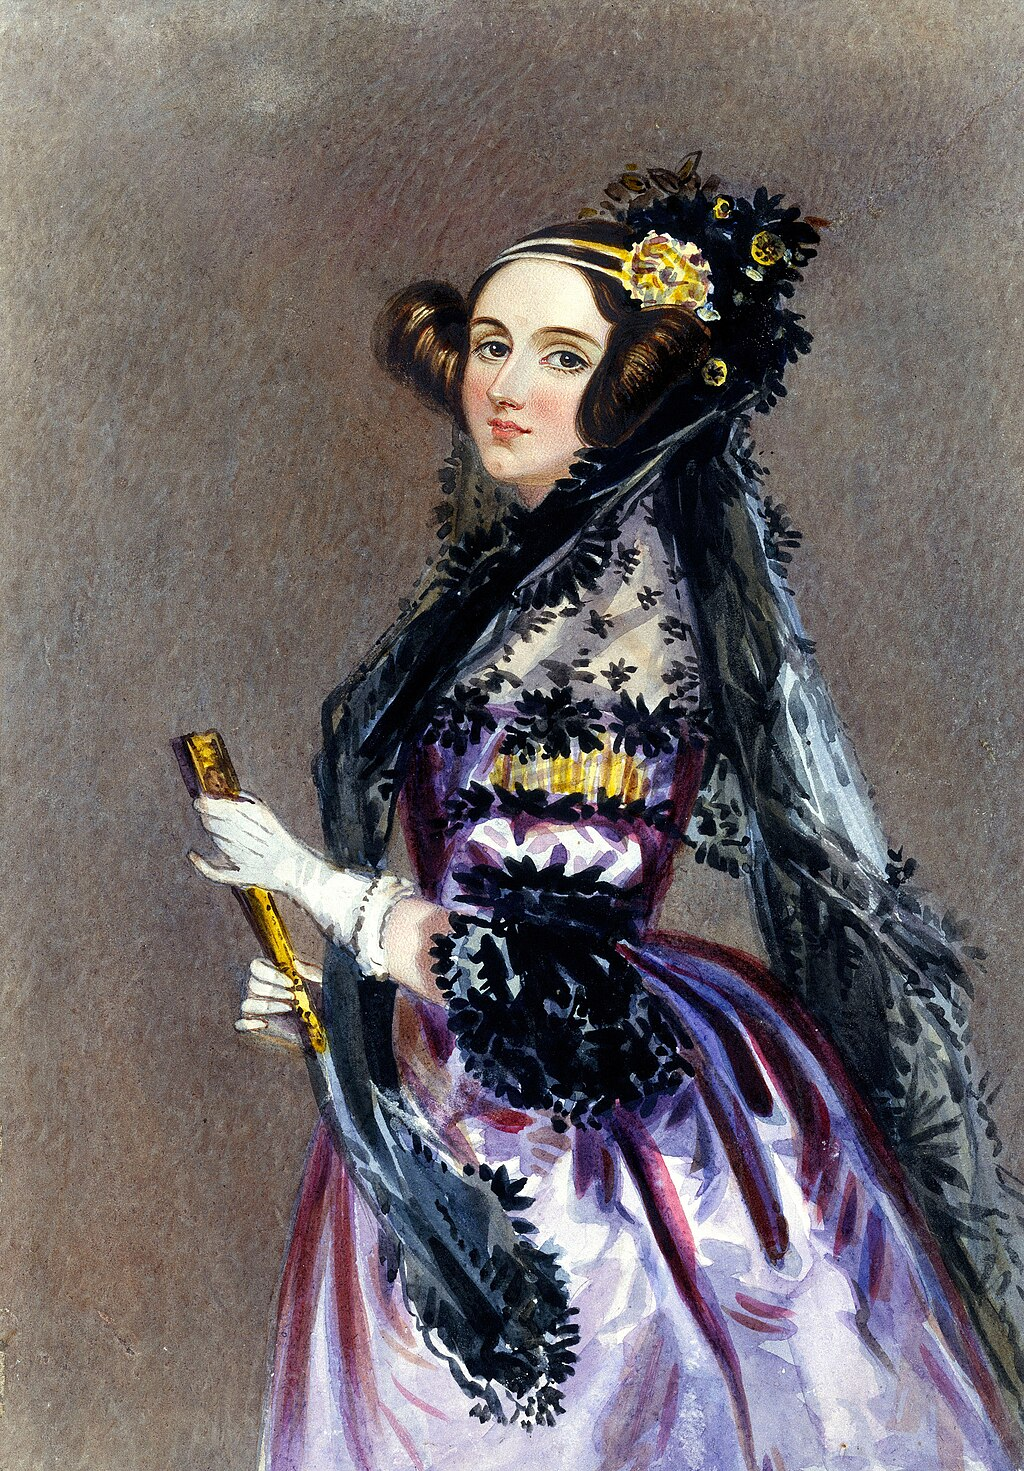
\includegraphics[width=0.3\textwidth]{images/Ada_Lovelace_portrait.jpg}
            \caption{Portrait of Ada Lovelace}
        \end{figure}
\end{frame}

\begin{frame}[t]{1843: Ada Lovelace - The First Programmer}
        \begin{itemize}
            \item Collaborated with Charles Babbage on his \textbf{Analytical Engine}
            \item The Thrilling Adventures of Lovelace and Babbage
        \end{itemize}


        \begin{figure}[b]
        \centering
          \subfloat[Trial Model of Analytical Machine]{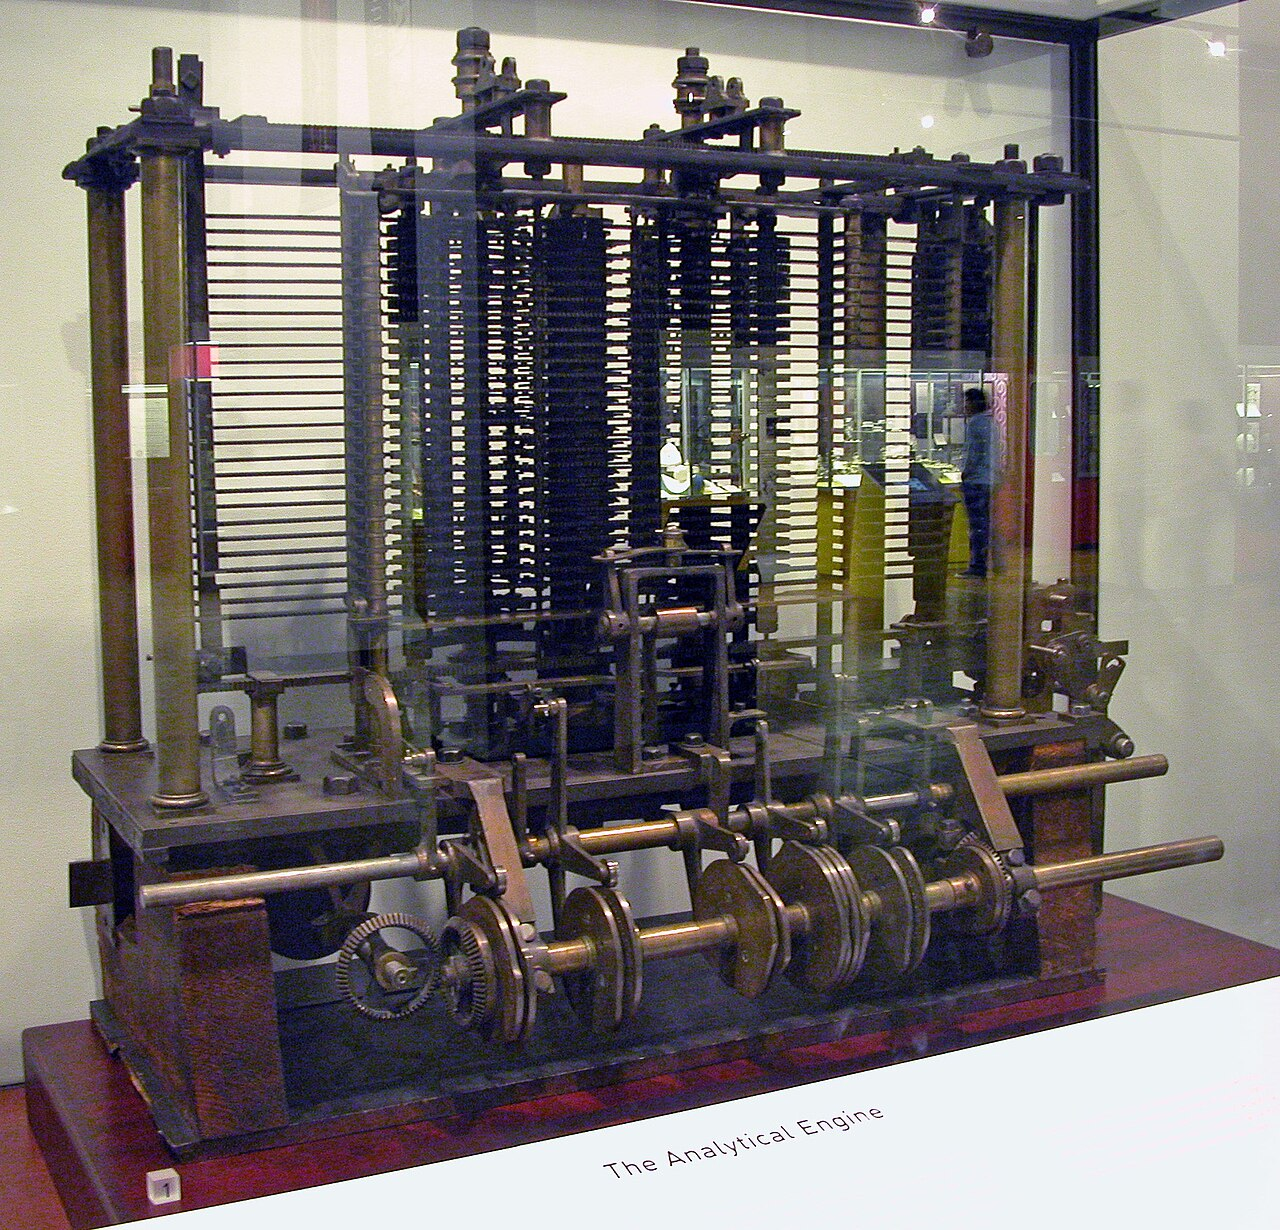
\includegraphics[height=4cm]{images/AnalyticalMachine_Babbage_London.jpg}}\qquad    
          \subfloat[Cover of the Comic]{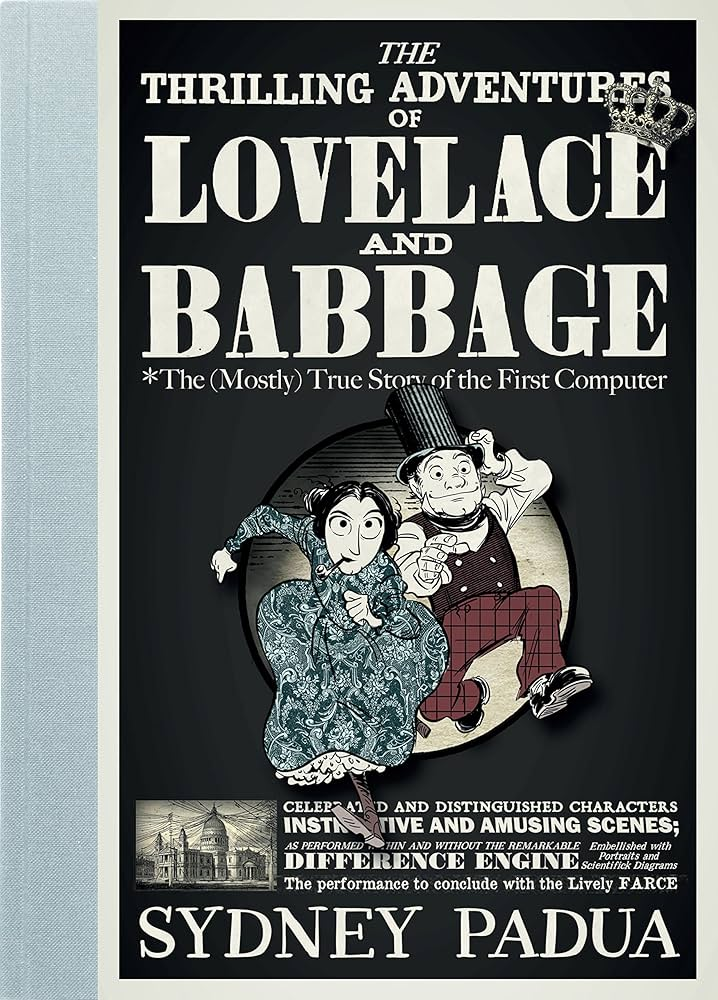
\includegraphics[height=4cm]{images/Comic_cover.jpg}}    

        % \subfloat[Trial Model of Analytical Machine]{
        %     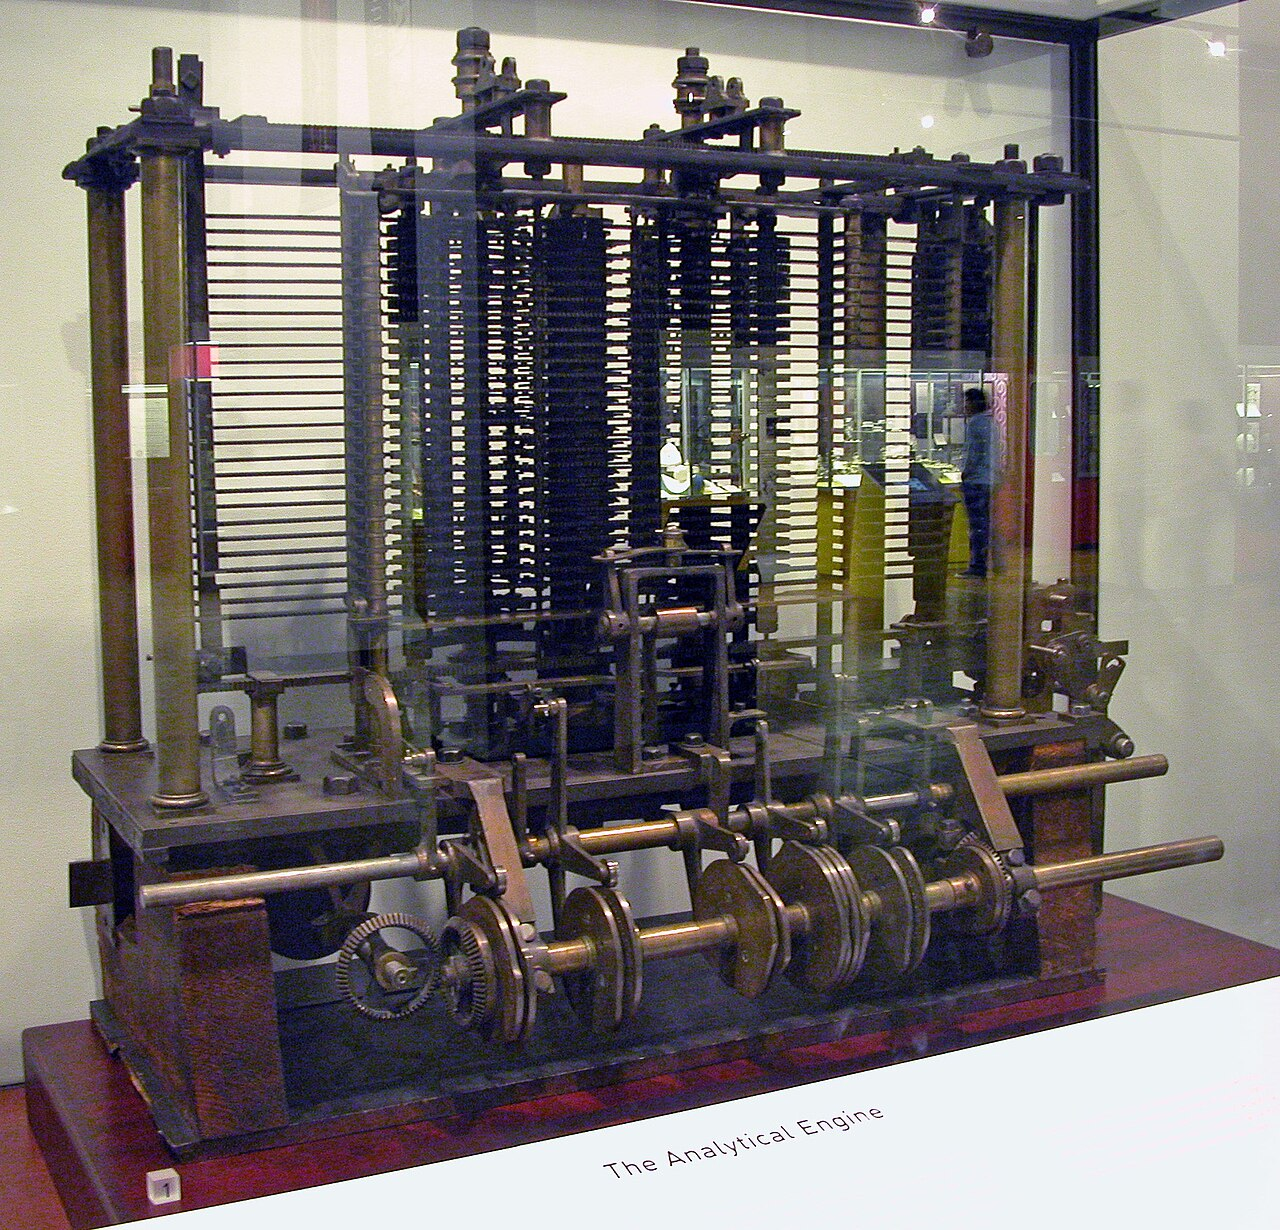
\includegraphics[width=0.3\textwidth]{images/AnalyticalMachine_Babbage_London.jpg}
        % }
        % \subfloat[Trial Model of Analytical Machine]{
        %     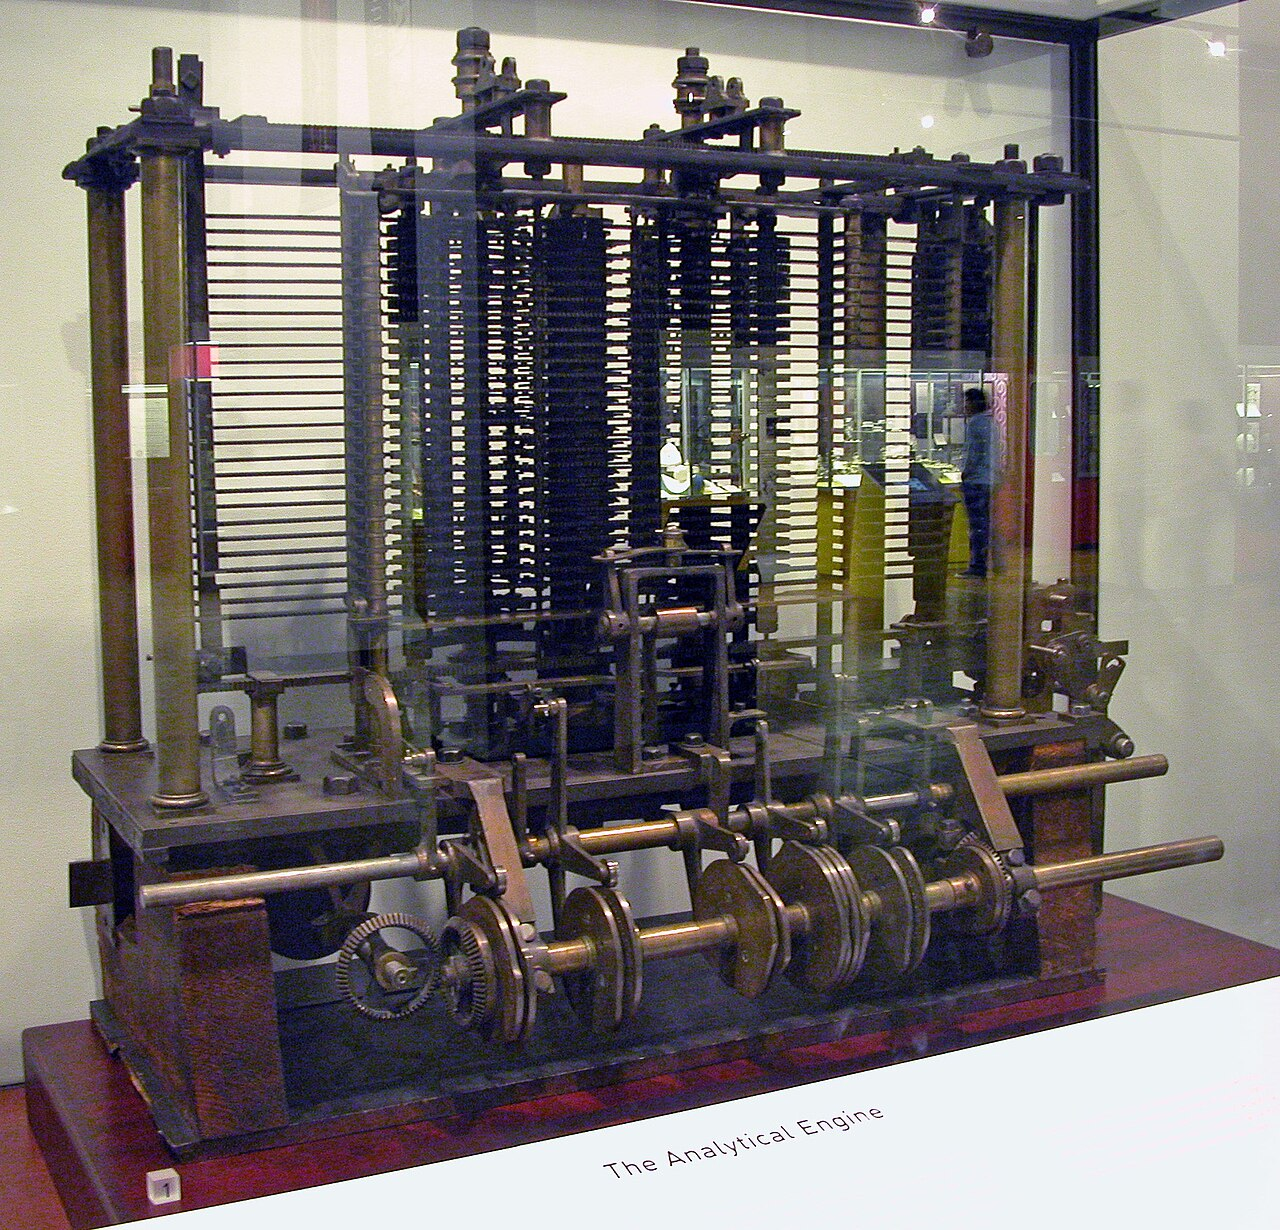
\includegraphics[width=0.3\textwidth]{images/AnalyticalMachine_Babbage_London.jpg}
        % }

        \caption{Analytical Machine}
        \end{figure}
\end{frame}

\begin{frame}[t]{1843: Ada Lovelace - The First Programmer}
        \begin{itemize}
            \item She translated an Italian article on the engine, adding her own extensive \textbf{Notes}
            \item \textbf{Note G} contained what is considered the first computer program
        \end{itemize}
        \begin{figure}[b]
            \centering
            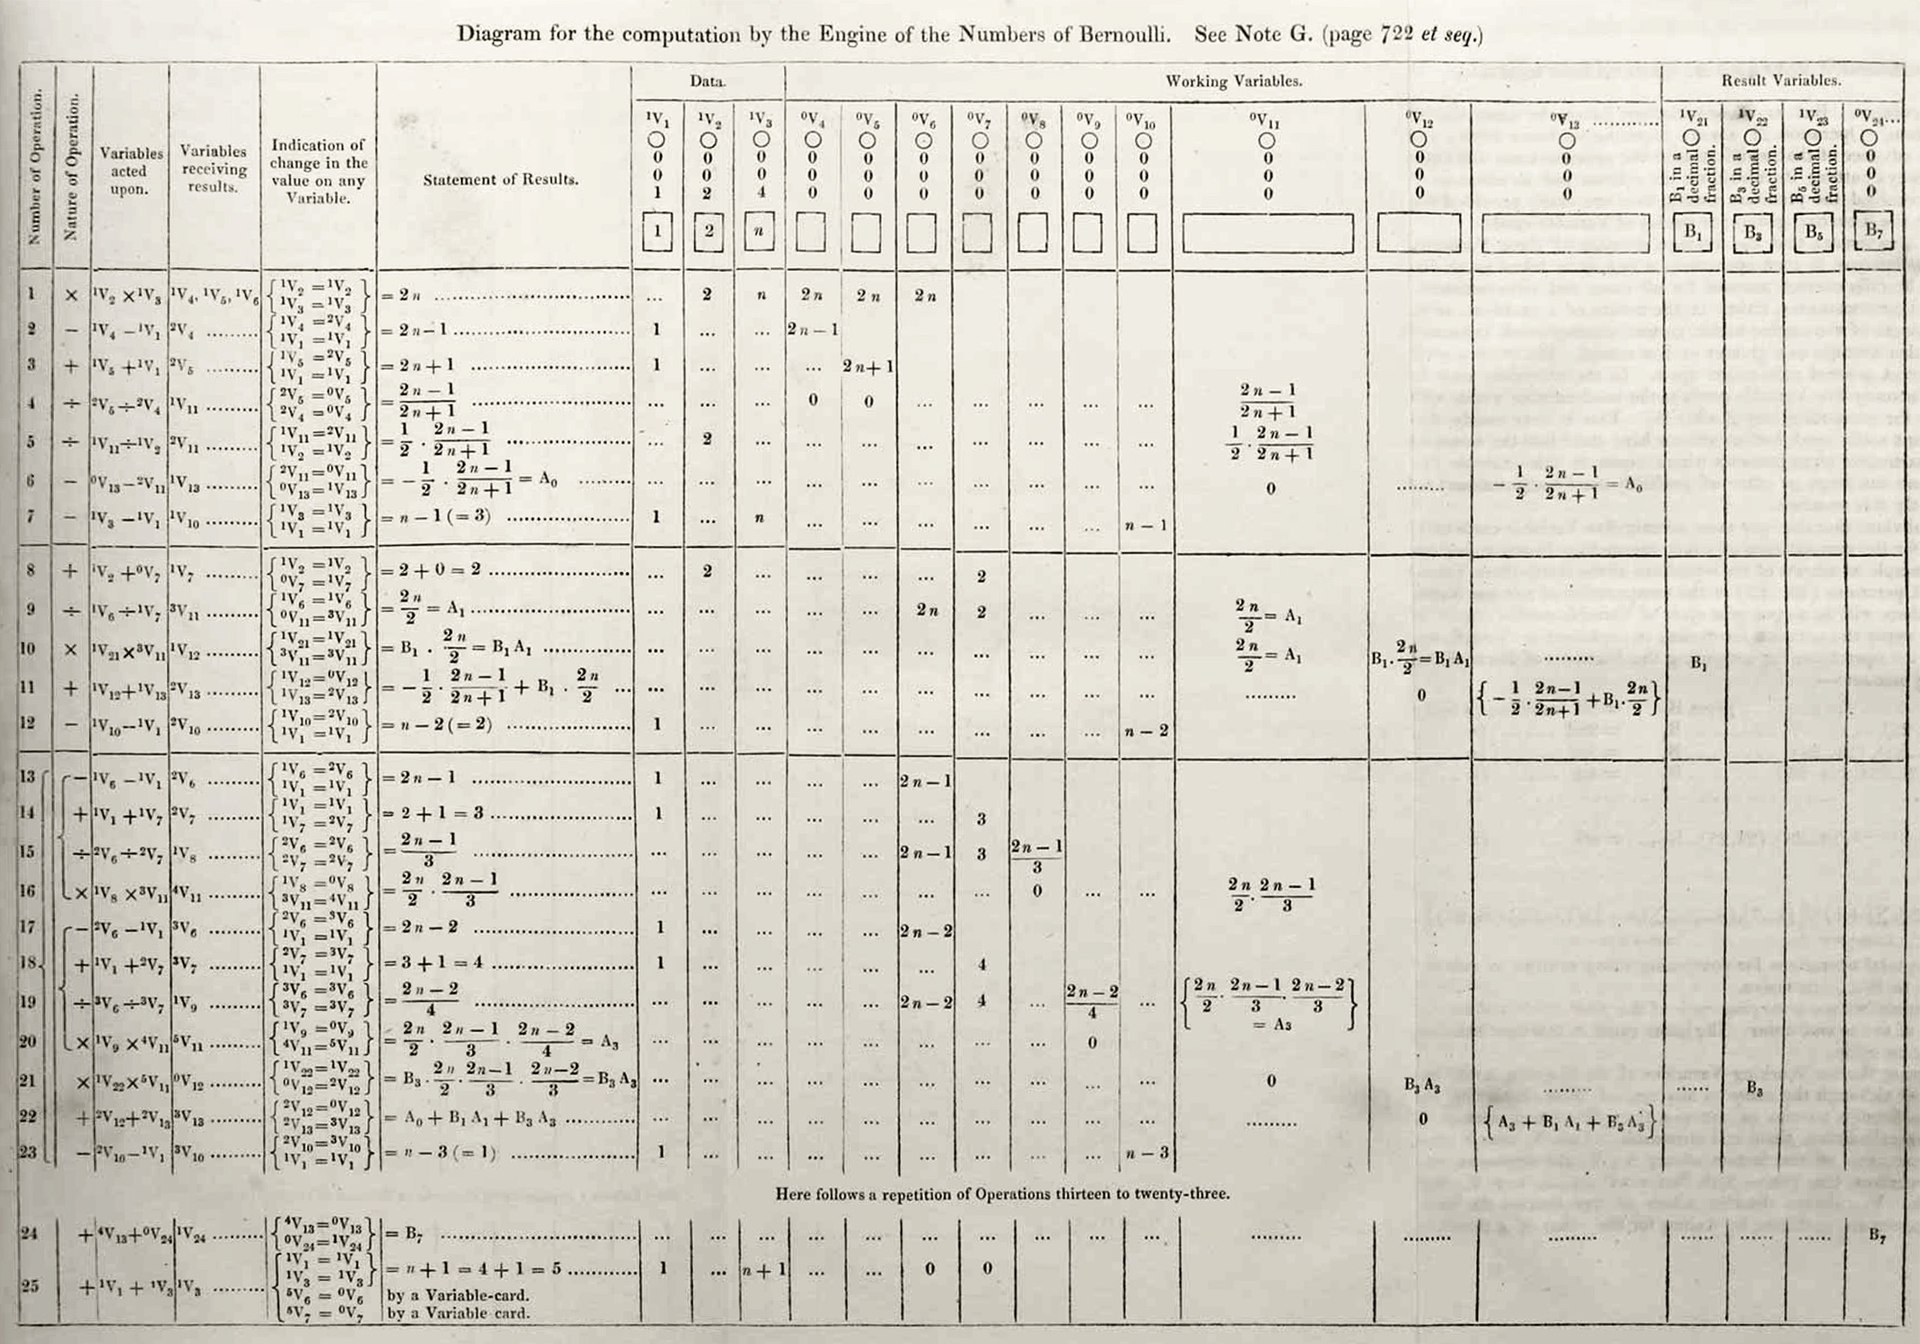
\includegraphics[width=0.5\textwidth]{images/Diagram_for_the_computation_of_Bernoulli_numbers.jpg}
            \caption{The First Program}
        \end{figure}
\end{frame}


% 第三页:遗产与影响
\begin{frame}[t]{Lovelace's Legacy}
\begin{itemize}
    \item \textbf{The Ada Programming Language}: Named in her honor by the US Department of Defense (1980). Designed for large-scale, safety-critical systems.
    \item \textbf{Ada Lovelace Day}: An international celebration held every second Tuesday of October.
\end{itemize}


    \begin{figure}[b]
        \centering
        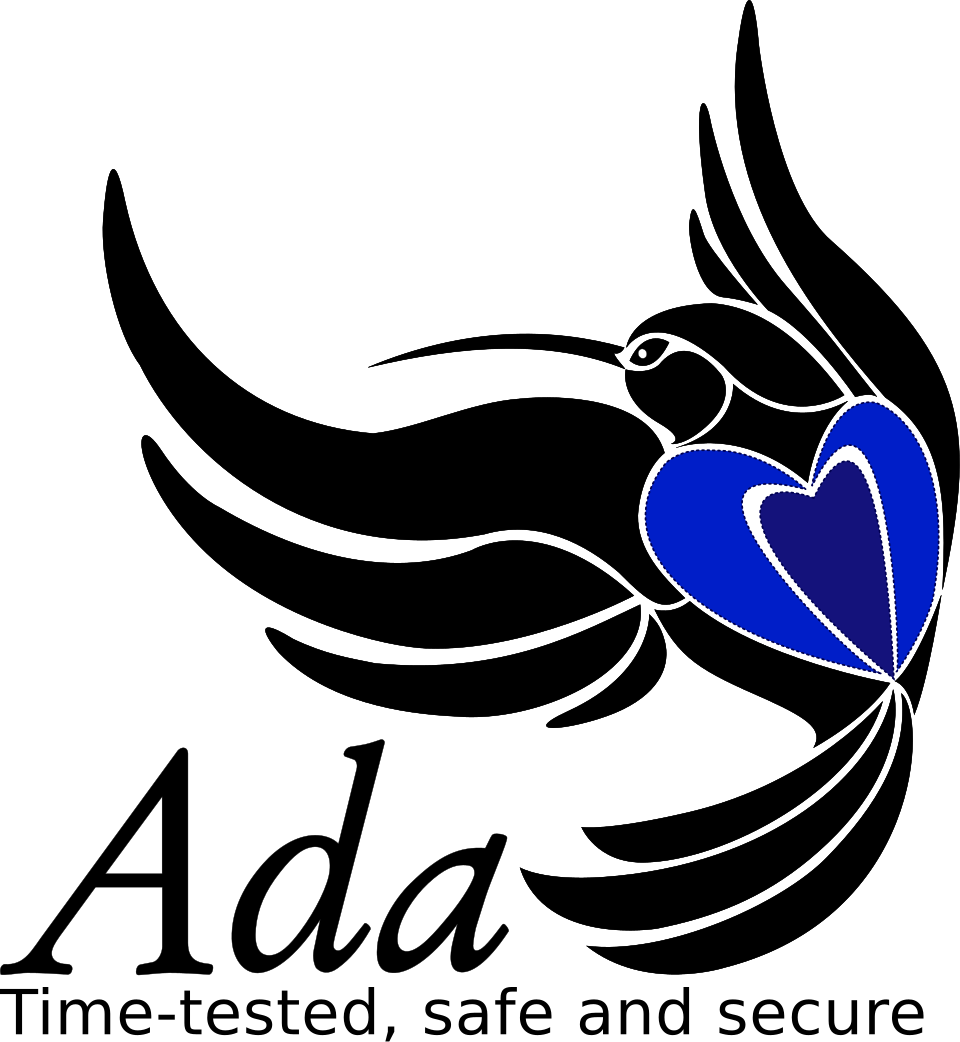
\includegraphics[width=0.3\textwidth]{images/Ada_logo.png}
        \caption{The Ada Programming Language Mascot}
    \end{figure}
\end{frame}

% 过渡幻灯片:从思想到实践
\begin{frame}[t]{From Vision to Reality}
\begin{center}
    \begin{tabular}{c}
        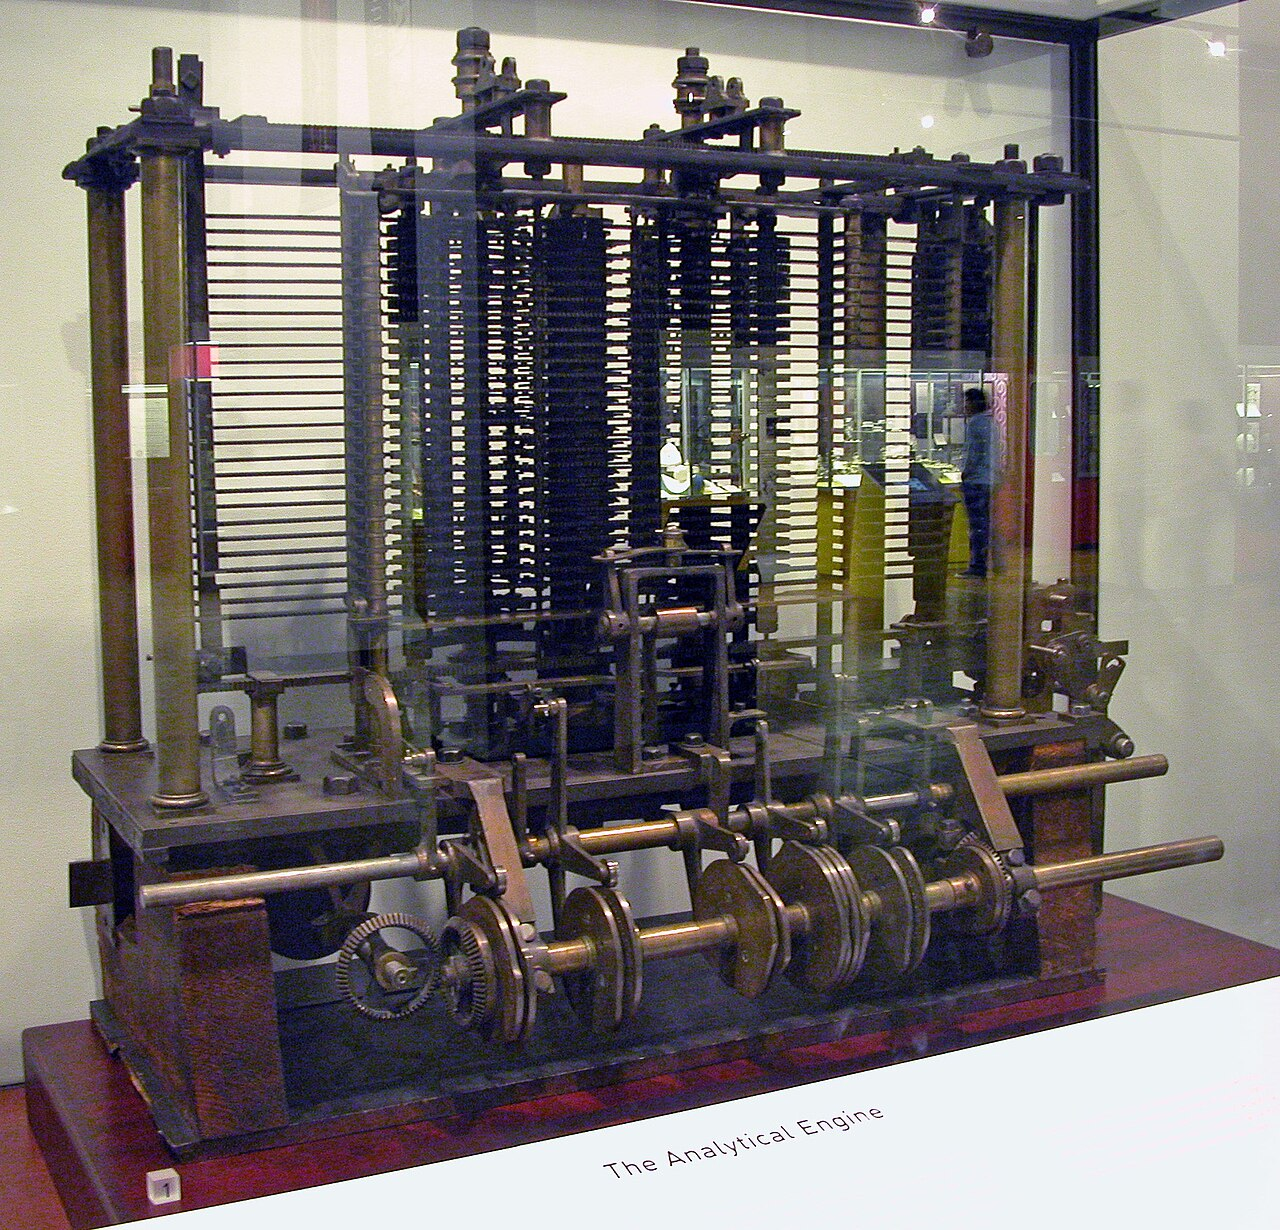
\includegraphics[width=0.25\textwidth]{images/AnalyticalMachine_Babbage_London.jpg} \\
        \textbf{1840s} Lovelace's Theoretical Program \\
        $\Downarrow$ \textbf{~100 Years} $\Downarrow$ \\
        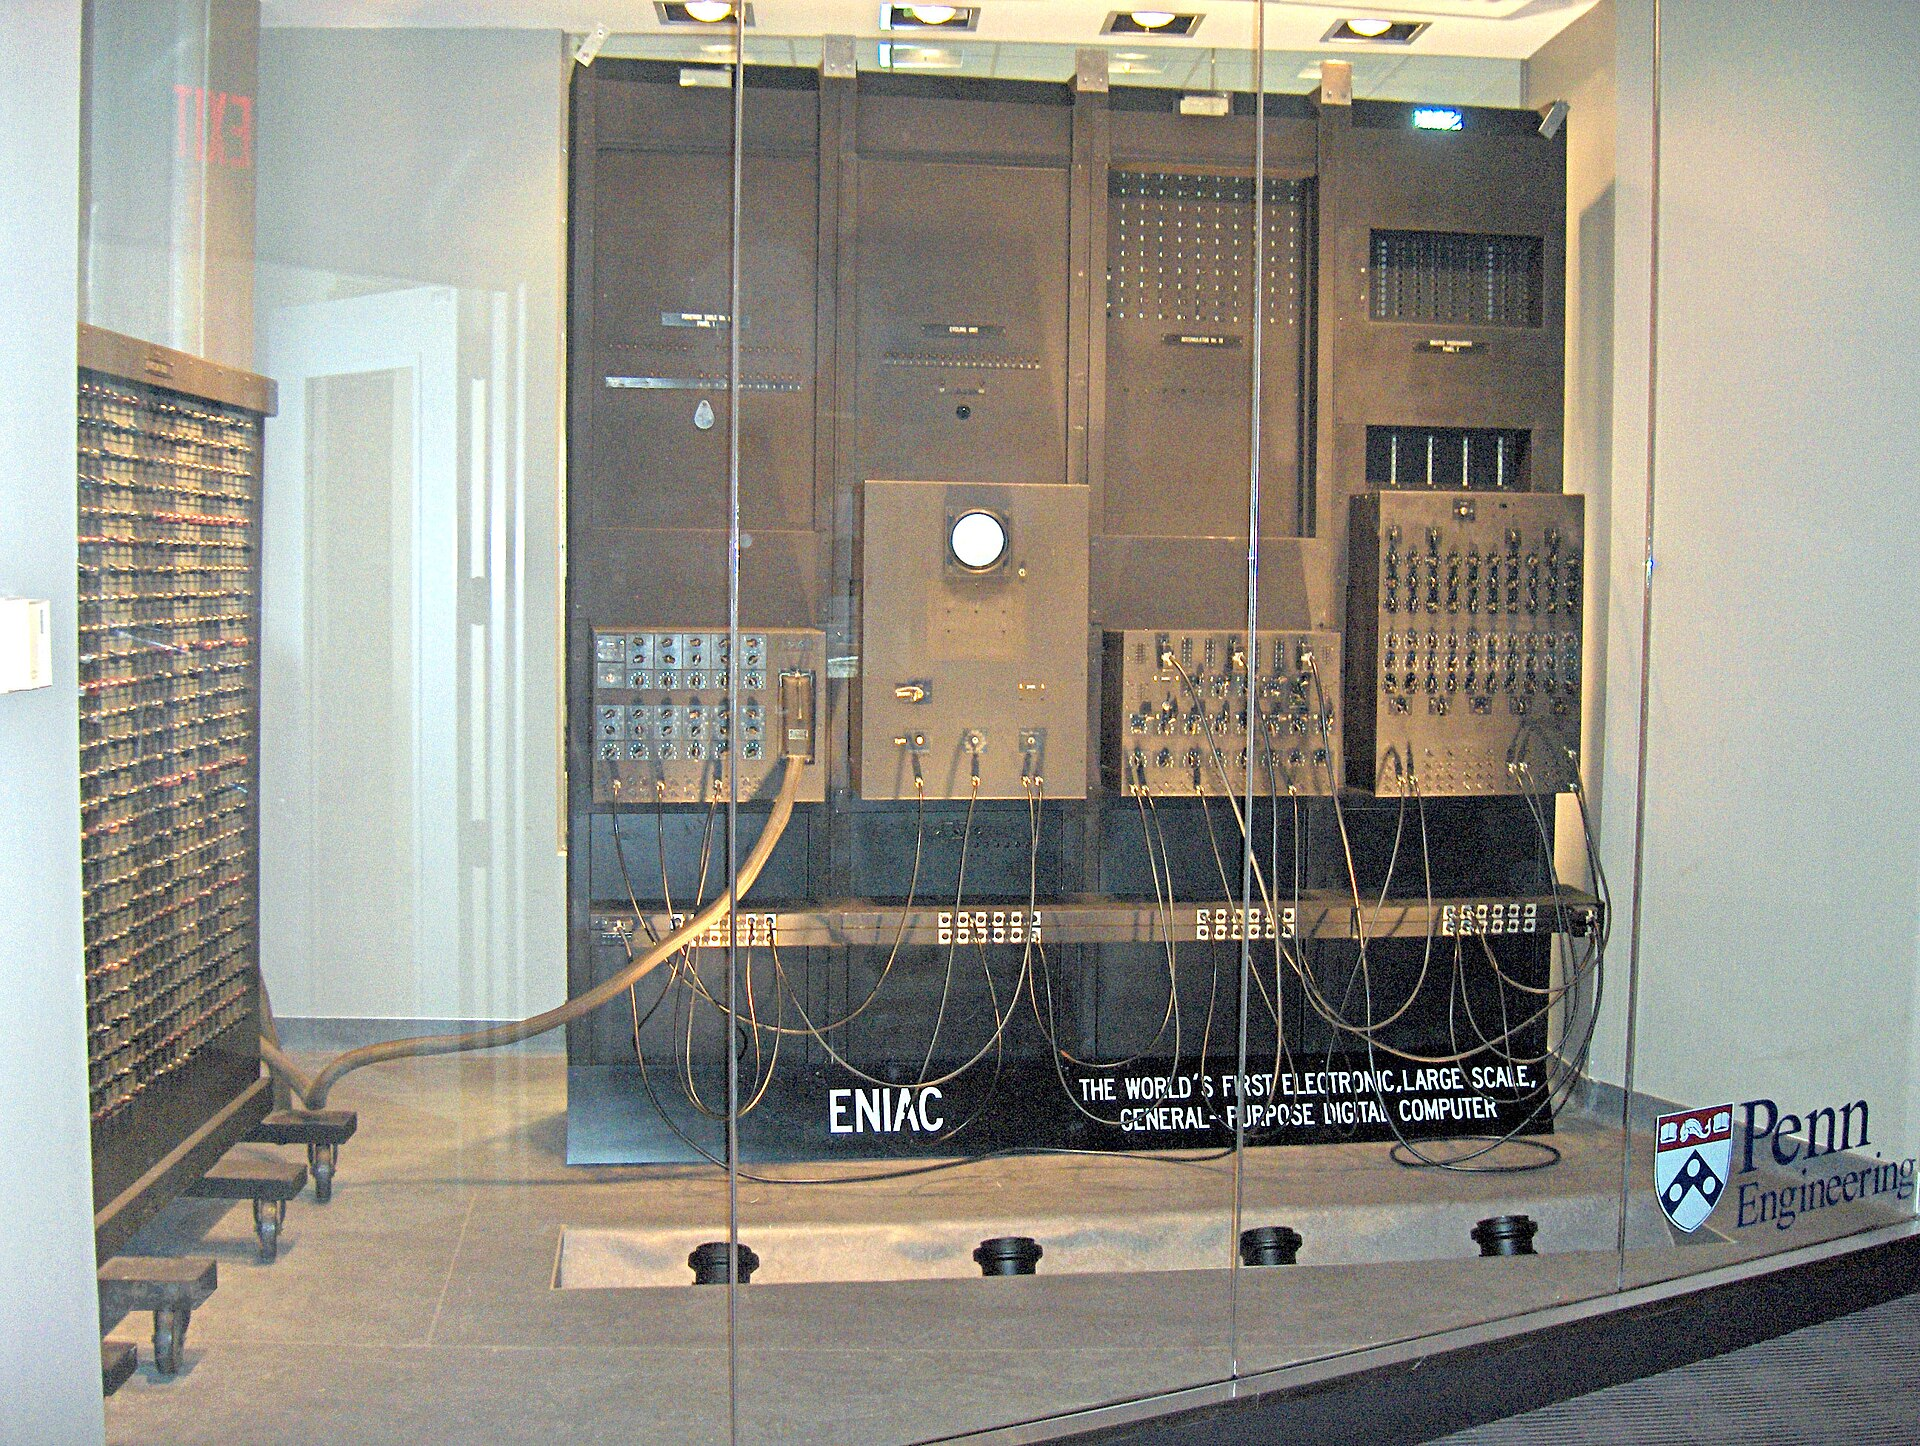
\includegraphics[width=0.25\textwidth]{images/ENIAC_Penn1.jpg} \\
        \textbf{1940s} ENIAC - First Electronic Computer \\
        % $\Downarrow$ \\
        % \includegraphics[width=0.3\textwidth]{images/nato1968_small.jpg} \\
        % \textbf{1968} \\
        % Software Engineering Born
    \end{tabular}
\end{center}
\end{frame}

\begin{frame}[t]
\frametitle{The Dawn of High-Level Programming}
\begin{itemize}
    \item \textbf{1950s Context}: Programming in machine code/assembly was tedious and error-prone
    \item \textbf{The Vision}: Create languages that were more human-readable and machine-independent
    \item \textbf{Two Paths Emerged}:
    \begin{itemize}
        \item \textbf{Fortran (1957)}: Designed for scientific computing - \textit{imperative} approach
        \item \textbf{Lisp (1958)}: Designed for AI research - \textit{functional} approach
    \end{itemize}
    \item Both languages are still actively used today, demonstrating remarkable longevity
\end{itemize}

\begin{center}
    \includegraphics[width=0.3\textwidth]{example-image}
    \quad
    \includegraphics[width=0.3\textwidth]{example-image}
    \\\scriptsize{Left: Early Fortran manual; Right: John McCarthy, Lisp creator}
\end{center}
\end{frame}

\begin{frame}[t]
\frametitle{Fortran: The First High-Level Language}
\begin{itemize}
    \item \textbf{Name}: FORmula TRANslating system
    \item \textbf{Created}: 1957 by John Backus at IBM
    \item \textbf{Primary Goal}: Make scientific computing easier and more efficient
    \item \textbf{Key Innovations}:
    \begin{itemize}
        \item First compiler ever created
        \item Mathematical notation similar to algebra
        \item Array operations and complex numbers
        \item Surprisingly efficient code generation
    \end{itemize}
    \item \textbf{Impact}: Revolutionized scientific and engineering computing
\end{itemize}

% \begin{block}{Backus' Insight}
% "Much of my work has come from being lazy. I didn't like writing programs, and so, when I was working on the IBM 701, I started work on a programming system to make it easier to write programs."
% \end{block}
\end{frame}

\begin{frame}[fragile,t]
\frametitle{Fortran Code Example}
\begin{lstlisting}[language=Fortran, caption=Fortran 77 Style]
\scriptsize
C AREA OF A TRIANGLE WITH HERON'S FORMULA
      PROGRAM TRIANGLE
      REAL A, B, C, AREA, S
      
      READ *, A, B, C
      S = (A + B + C) / 2.0
      AREA = SQRT(S * (S - A) * (S - B) * (S - C))
      
      PRINT *, 'AREA = ', AREA
      END PROGRAM
\end{lstlisting}

\begin{itemize}
    \item \textbf{Imperative style}: Explicit sequence of operations
    \item \textbf{Mathematical focus}: Direct translation of formulas
    \item \textbf{Simple data flow}: Variables are modified in place
    \item \textbf{Fixed format}: Early versions required specific column positions
\end{itemize}
\end{frame}

\begin{frame}[t]
\frametitle{Lisp: The Second High-Level Language}
\begin{itemize}
    \item \textbf{Name}: LISt Processing
    \item \textbf{Created}: 1958 by John McCarthy at MIT
    \item \textbf{Primary Goal}: Artificial Intelligence research
    \item \textbf{Key Innovations}:
    \begin{itemize}
        \item Functional programming paradigm
        \item Linked list as fundamental data structure
        \item Garbage collection
        \item Homoiconicity: Code is data, data is code
        \item Recursion as primary control structure
    \end{itemize}
    \item \textbf{Impact}: Foundation for AI research and functional programming
\end{itemize}

% \begin{block}{McCarthy's Vision}
% "Lisp was a discovery, not an invention. It was there, in the nature of recursive functions of symbolic expressions."
% \end{block}
\end{frame}

\begin{frame}[fragile,t]
\frametitle{Lisp Code Example}
\scriptsize
\begin{lstlisting}[language=Lisp, caption=Common Lisp Style]
;; Calculate factorial using recursion
(defun factorial (n)
  (if (<= n 1)
      1
      (* n (factorial (- n 1)))))

;; Map a function over a list
(defun square-list (numbers)
  (mapcar #'(lambda (x) (* x x)) numbers))

;; Using higher-order functions
(let ((numbers '(1 2 3 4 5)))
  (print (factorial 5))
  (print (square-list numbers)))
\end{lstlisting}

\begin{itemize}
    \item \textbf{Functional style}: Emphasizes expressions over statements
    \item \textbf{Recursive thinking}: Problems broken down recursively
    \item \textbf{List manipulation}: Built-in operations for list processing
\end{itemize}
\end{frame}

\begin{frame}[t]
\frametitle{Paradigm Comparison: Imperative vs Functional}
\begin{itemize}
    \item \textbf{Fortran (Imperative Paradigm)}:
    \begin{itemize}
        \item \textit{Philosophy}: "How to compute" - sequence of steps
        \item \textit{State changes}: Variables are modified
        \item \textit{Control structures}: Loops, conditionals, goto
        \item \textit{Primary abstraction}: Procedures and subroutines
        \item \textit{Memory management}: Manual/stack-based
    \end{itemize}
    
    \item \textbf{Lisp (Functional Paradigm)}:
    \begin{itemize}
        \item \textit{Philosophy}: "What to compute" - expressions and transformations
        \item \textit{Immutability}: Avoid changing state when possible
        \item \textit{Control structures}: Recursion, function composition
        \item \textit{Primary abstraction}: Functions as first-class citizens
        \item \textit{Memory management}: Automatic garbage collection
    \end{itemize}
\end{itemize}
\end{frame}

\begin{frame}[t]
\frametitle{Design Philosophy Comparison}
\begin{itemize}
    \item \textbf{Fortran's Practical Focus}:
    \begin{itemize}
        \item Designed for numerical computation efficiency
        \item Close mapping to mathematical notation
        \item Optimized for array operations and linear algebra
        \item Minimal syntax, maximum computational power
        \item Target user: Scientists and engineers
    \end{itemize}
    
    \item \textbf{Lisp's Theoretical Foundation}:
    \begin{itemize}
        \item Based on lambda calculus and recursive function theory
        \item Embraced symbolic computation and AI problems
        \item Powerful metaprogramming through macros
        \item Interactive development with REPL (Read-Eval-Print Loop)
        \item Target user: AI researchers and computer scientists
    \end{itemize}
\end{itemize}
\end{frame}


\subsection{The Origins}

\begin{frame}[t]{The Dawn of Software Engineering}
\begin{itemize}
    \item \textbf{1968 NATO Conference}: The term "Software Engineering" 
    \item Addressing the "software crisis" - growing complexity and cost of software development
    \item Key goal: Apply engineering principles to software development
\end{itemize}
    \begin{figure}[b]
        \centering
        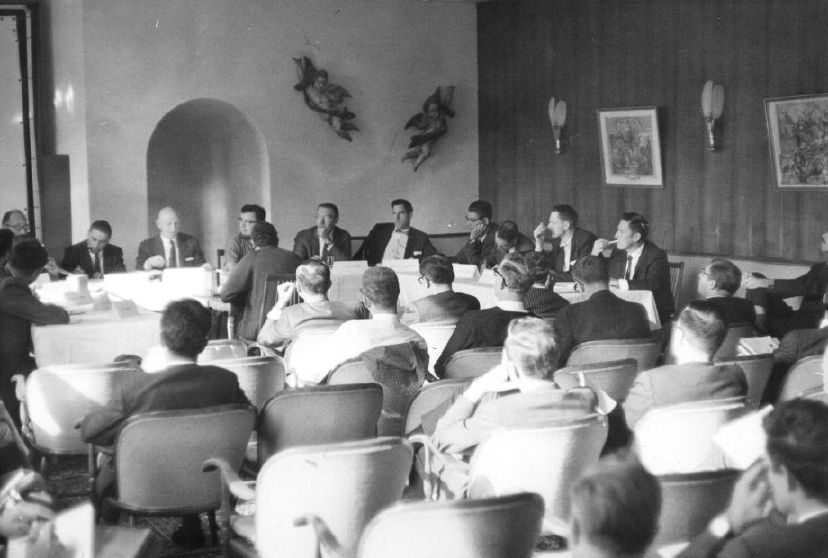
\includegraphics[width=0.3\textwidth]{images/NATO-conference-photo.png}
        \caption{The 1968 NATO Garmisch Conference}
    \end{figure}
\end{frame}

\subsection{Foundational Concepts}

\begin{frame}[t]{1968: "Goto Statement Considered Harmful"}
\begin{itemize}
    \item \textbf{Edsger Dijkstra's seminal letter} (1968)
    \item Advocated against use of GOTO statements
    \item Promoted structured programming principles
    \item Foundation for modern control structures (if-else, while, for)
    \item Emphasized code readability and maintainability
\end{itemize}
\begin{block}{Dijkstra's Insight}
"Program testing can be used to show the presence of bugs, but never to show their absence!"
\end{block}
\end{frame}

\begin{frame}[t]{1975: The Mythical Man-Month}
\begin{columns}
    \begin{column}{0.6\textwidth}
        \begin{itemize}
            \item \textbf{Frederick Brooks' seminal book} (1975)
            \item Based on experience managing IBM OS/360 development
            \item \textbf{Core thesis}: "Adding manpower to a late software project makes it later"
            \item \alert{Brooks's Law}: The "man-month" is a dangerous and fallacious unit of measurement for software work due to communication overhead.
            \item ``No Silver Bullet''
        \end{itemize}
    \end{column}
    \begin{column}{0.4\textwidth}
        % Placeholder for the book cover image
        % \includegraphics[width=0.9\textwidth]{images/man-month-cover.jpg}
        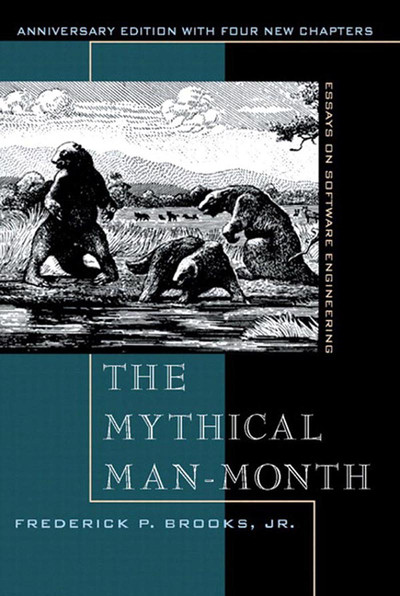
\includegraphics[width=0.6\textwidth]{images/Mythical Man-Month.jpg}
    \end{column}
\end{columns}
\end{frame}
% ========== END OF NEW SLIDE ==========

\subsection{Key Milestones}

\begin{frame}[t]{1984: Reflections on Trusting Trust}
\begin{itemize}
    \item \textbf{Ken Thompson's Turing Award Lecture} (1984)
    \item A compiler could insert backdoors that propagate themselves
    \item Fundamental insight into software supply chain security
\end{itemize}
\begin{figure}
    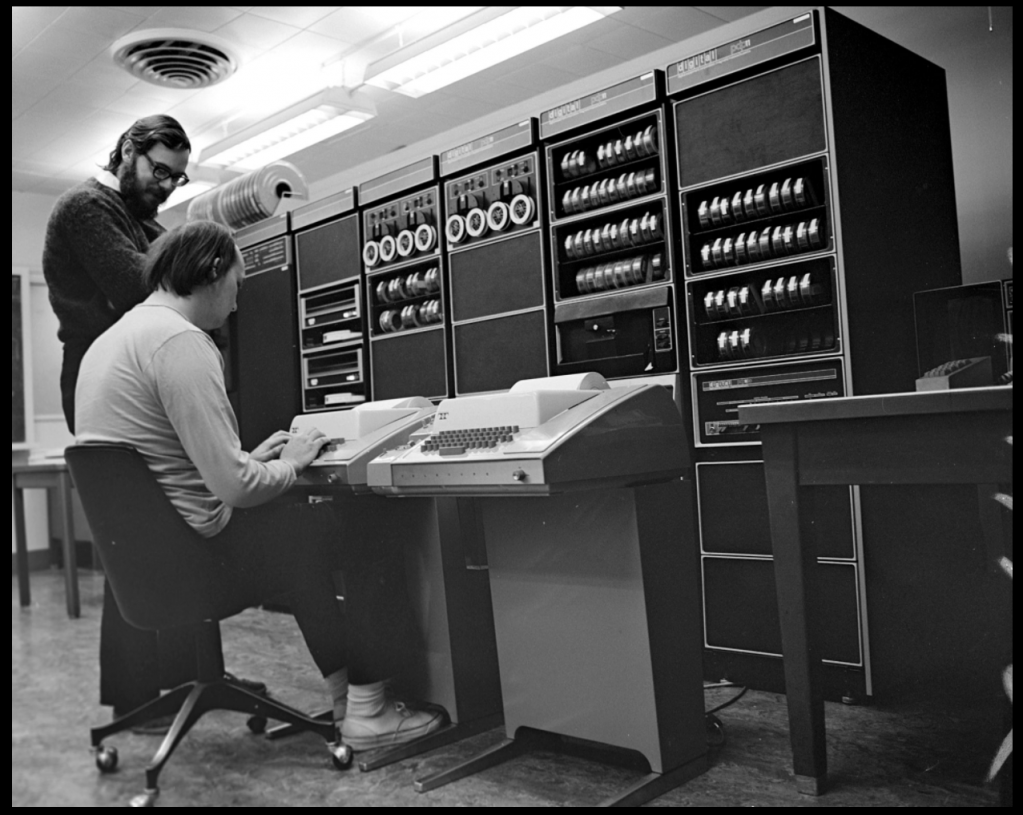
\includegraphics[width=0.3\textwidth]{images/Ken_UNIX.png}
    \caption{Ken Thompson and Dennis Ritchie with UNIX}
\end{figure}
\pause
\begin{alertblock}{Key Takeaway}
    The tools we use to build software must themselves be trustworthy. There is no ultimate root of trust.
\end{alertblock}
\end{frame}



\begin{frame}[t]{1980s-1990s: GNU and Open Source Revolution}
    \begin{itemize}
        \item \textbf{Richard Stallman launches GNU Project} (1983)
        \item Free Software Foundation established (1985)
    \end{itemize}
    \begin{figure}
        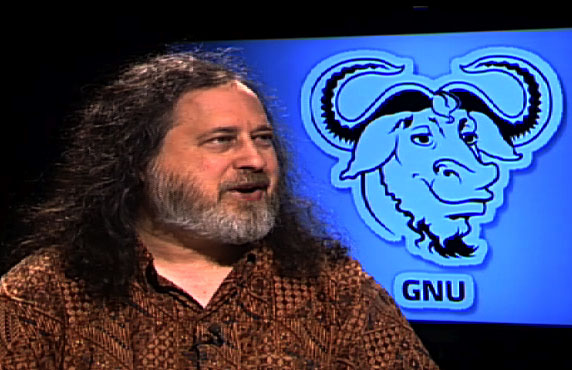
\includegraphics[width=0.8\textwidth]{images/stallman.jpg}
        \caption{Richard and the GNU project}
    \end{figure}
\end{frame}

\begin{frame}[t]{1980s-1990s: GNU and Open Source Revolution}
    \begin{itemize}
        \item Linux kernel created by Linus Torvalds (1991)
        \item Open Source Initiative founded (1998)
    \end{itemize}
    \begin{figure}
        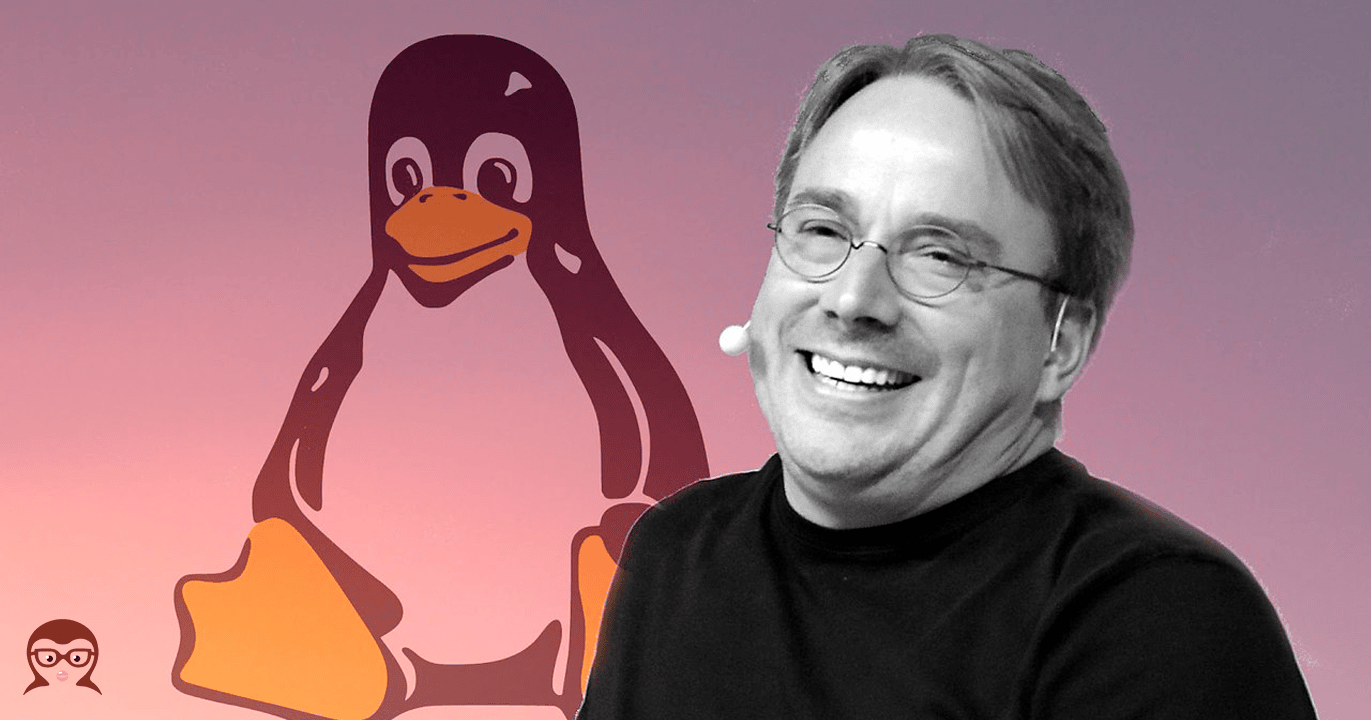
\includegraphics[width=0.8\textwidth]{images/Linus-Torvalds-Linux.png}
        \caption{Linus Torvalds and Linux}
    \end{figure}
\end{frame}

\begin{frame}[t]{From Netscape to Firefox}

\begin{block}{The Fall of a Giant: Netscape's ``Cathedral''}
\begin{itemize}
    \item \textbf{Netscape Navigator} dominated the early web with 90\% market share in the mid-1990s.
    \item Lost the "first browser war" to Microsoft's Internet Explorer (bundled with Windows).
    \item Facing irrelevance, Netscape took a radical step in \textbf{1998}.
\end{itemize}
\end{block}
\end{frame}

\begin{frame}[t]{From Netscape to Firefox}
\begin{block}{The Radical Shift: Embracing the ``Bazaar''}
\begin{itemize}
    \item In January 1998, Netscape \textbf{open-sourced} its browser code (Netscape Communicator 4.0) to harness the power of distributed developers.
    \item The \textbf{Mozilla Organization} was created to manage the project.
    \item The old code was unwieldy; developers started from scratch with the new \textbf{Gecko} rendering engine.
\end{itemize}
\end{block}

\end{frame}

\begin{frame}[t]{From Netscape to Firefox}
\begin{block}{The Phoenix Rises: Birth of Firefox}
\begin{itemize}
    \item From the Mozilla codebase, a lightweight, user-focused browser emerged named \textbf{Phoenix} (2002).
    \item After trademark disputes (Phoenix $\rightarrow$ Firebird $\rightarrow$ \textbf{Firefox}), Mozilla Firefox 1.0 launched in \textbf{2004}.
    \item Firefox challenged IE's monopoly, championing open standards and user choice.
\end{itemize}
\end{block}

\end{frame}

\begin{frame}[t]{The Philosophical Engine: Cathedral vs. Bazaar}

\begin{columns}
    \begin{column}{0.48\textwidth}
        \begin{block}{Cathedral Model}
            \scriptsize
            \begin{itemize}
                \item \textbf{Closed, centralized development}.
                \item Built by a small, dedicated team of experts.
                \item Releases are infrequent, grand events.
                \item \textbf{Examples}: Pre-1998 Netscape, traditional software development.
            \end{itemize}
        \end{block}
    \end{column}
    \begin{column}{0.48\textwidth}
        \begin{block}{Bazaar Model}
            \scriptsize
            \begin{itemize}
                \item \textbf{Open, decentralized development}.
                \item Code is developed publicly over the Internet.
                \item "Given enough eyeballs, all bugs are shallow."
                \item \textbf{Examples}: Mozilla, Linux, Firefox.
            \end{itemize}
        \end{block}
    \end{column}
\end{columns}

\vspace{1em}

\begin{exampleblock}{The Core Lesson}
The Netscape-to-Firefox story shows that a well-managed \textbf{Bazaar} model can build complex, high-quality systems (a "cathedral") more effectively than a closed model by leveraging global collaboration.
\end{exampleblock}

\end{frame}

\begin{frame}[t]{Legacy and Lasting Impact}
\begin{itemize}
    \item \textbf{Technical Foundations}: The Gecko engine paved the way for Firefox. Netscape's legacy also includes JavaScript, SSL, and Cookies, invented by its engineers.
    \item \textbf{Institutionalization}: The \textbf{Mozilla Foundation} (est. July 15, 2003) ensures the project's mission continues beyond any single company.
    \item \textbf{A Lasting Battle}: Firefox became the leading alternative to IE, proving the viability of open-source software for mainstream users and setting the stage for the modern web.
\end{itemize}

\begin{center}
    \textbf{The open-source bazaar, born from a cathedral's ashes, helped ensure the web remained open and competitive.}
\end{center}
\end{frame}

\begin{frame}[t]{1980s-1990s: Object-Oriented Revolution}
\begin{itemize}
    \item \textbf{Smalltalk} (1970s-1980s): Pure OOP concepts
    \item \textbf{C++} (1985): Bringing OOP to systems programming
    \item \textbf{Java} (1995): "Write once, run anywhere"
    \item Key principles: Encapsulation, Inheritance, Polymorphism
    \item Design Patterns (Gang of Four book, 1994)
\end{itemize}

\begin{figure}
    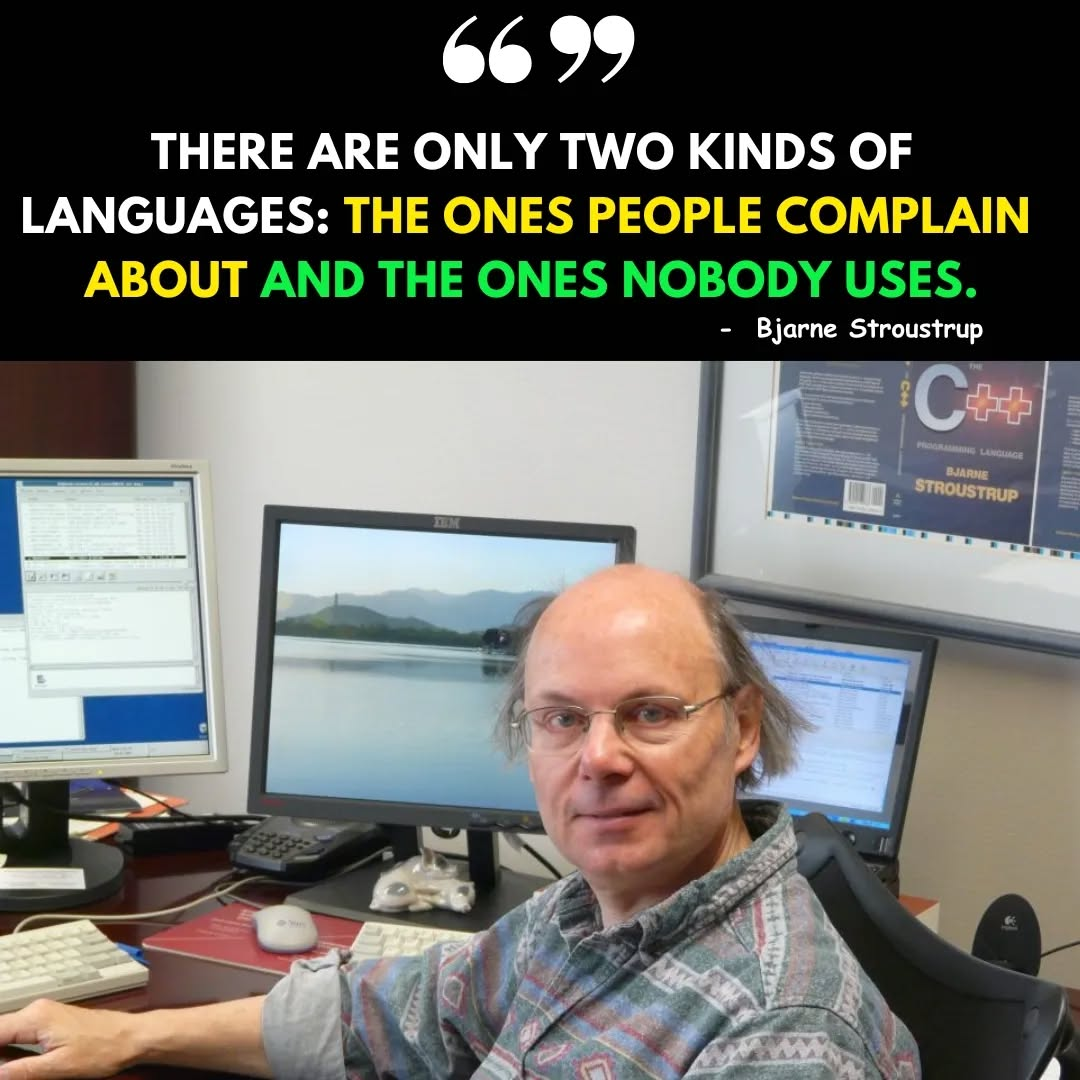
\includegraphics[width=0.3\textwidth]{images/cpp.jpeg}
    \caption{Quotes of the Creator of C++}
\end{figure}

\end{frame}

\subsection{Modern Era}

\begin{frame}[t]{2000s: Agile and DevOps}
    \begin{itemize}
        \item \textbf{Agile Manifesto} (2001):  Emphasis on iterative development and customer collaboration
        \item \textbf{DevOps movement} (late 2000s)
        \item Bridging development and operations, featuring Git and CI/CD
        \item Infrastructure as Code
    \end{itemize}
    \begin{figure}
        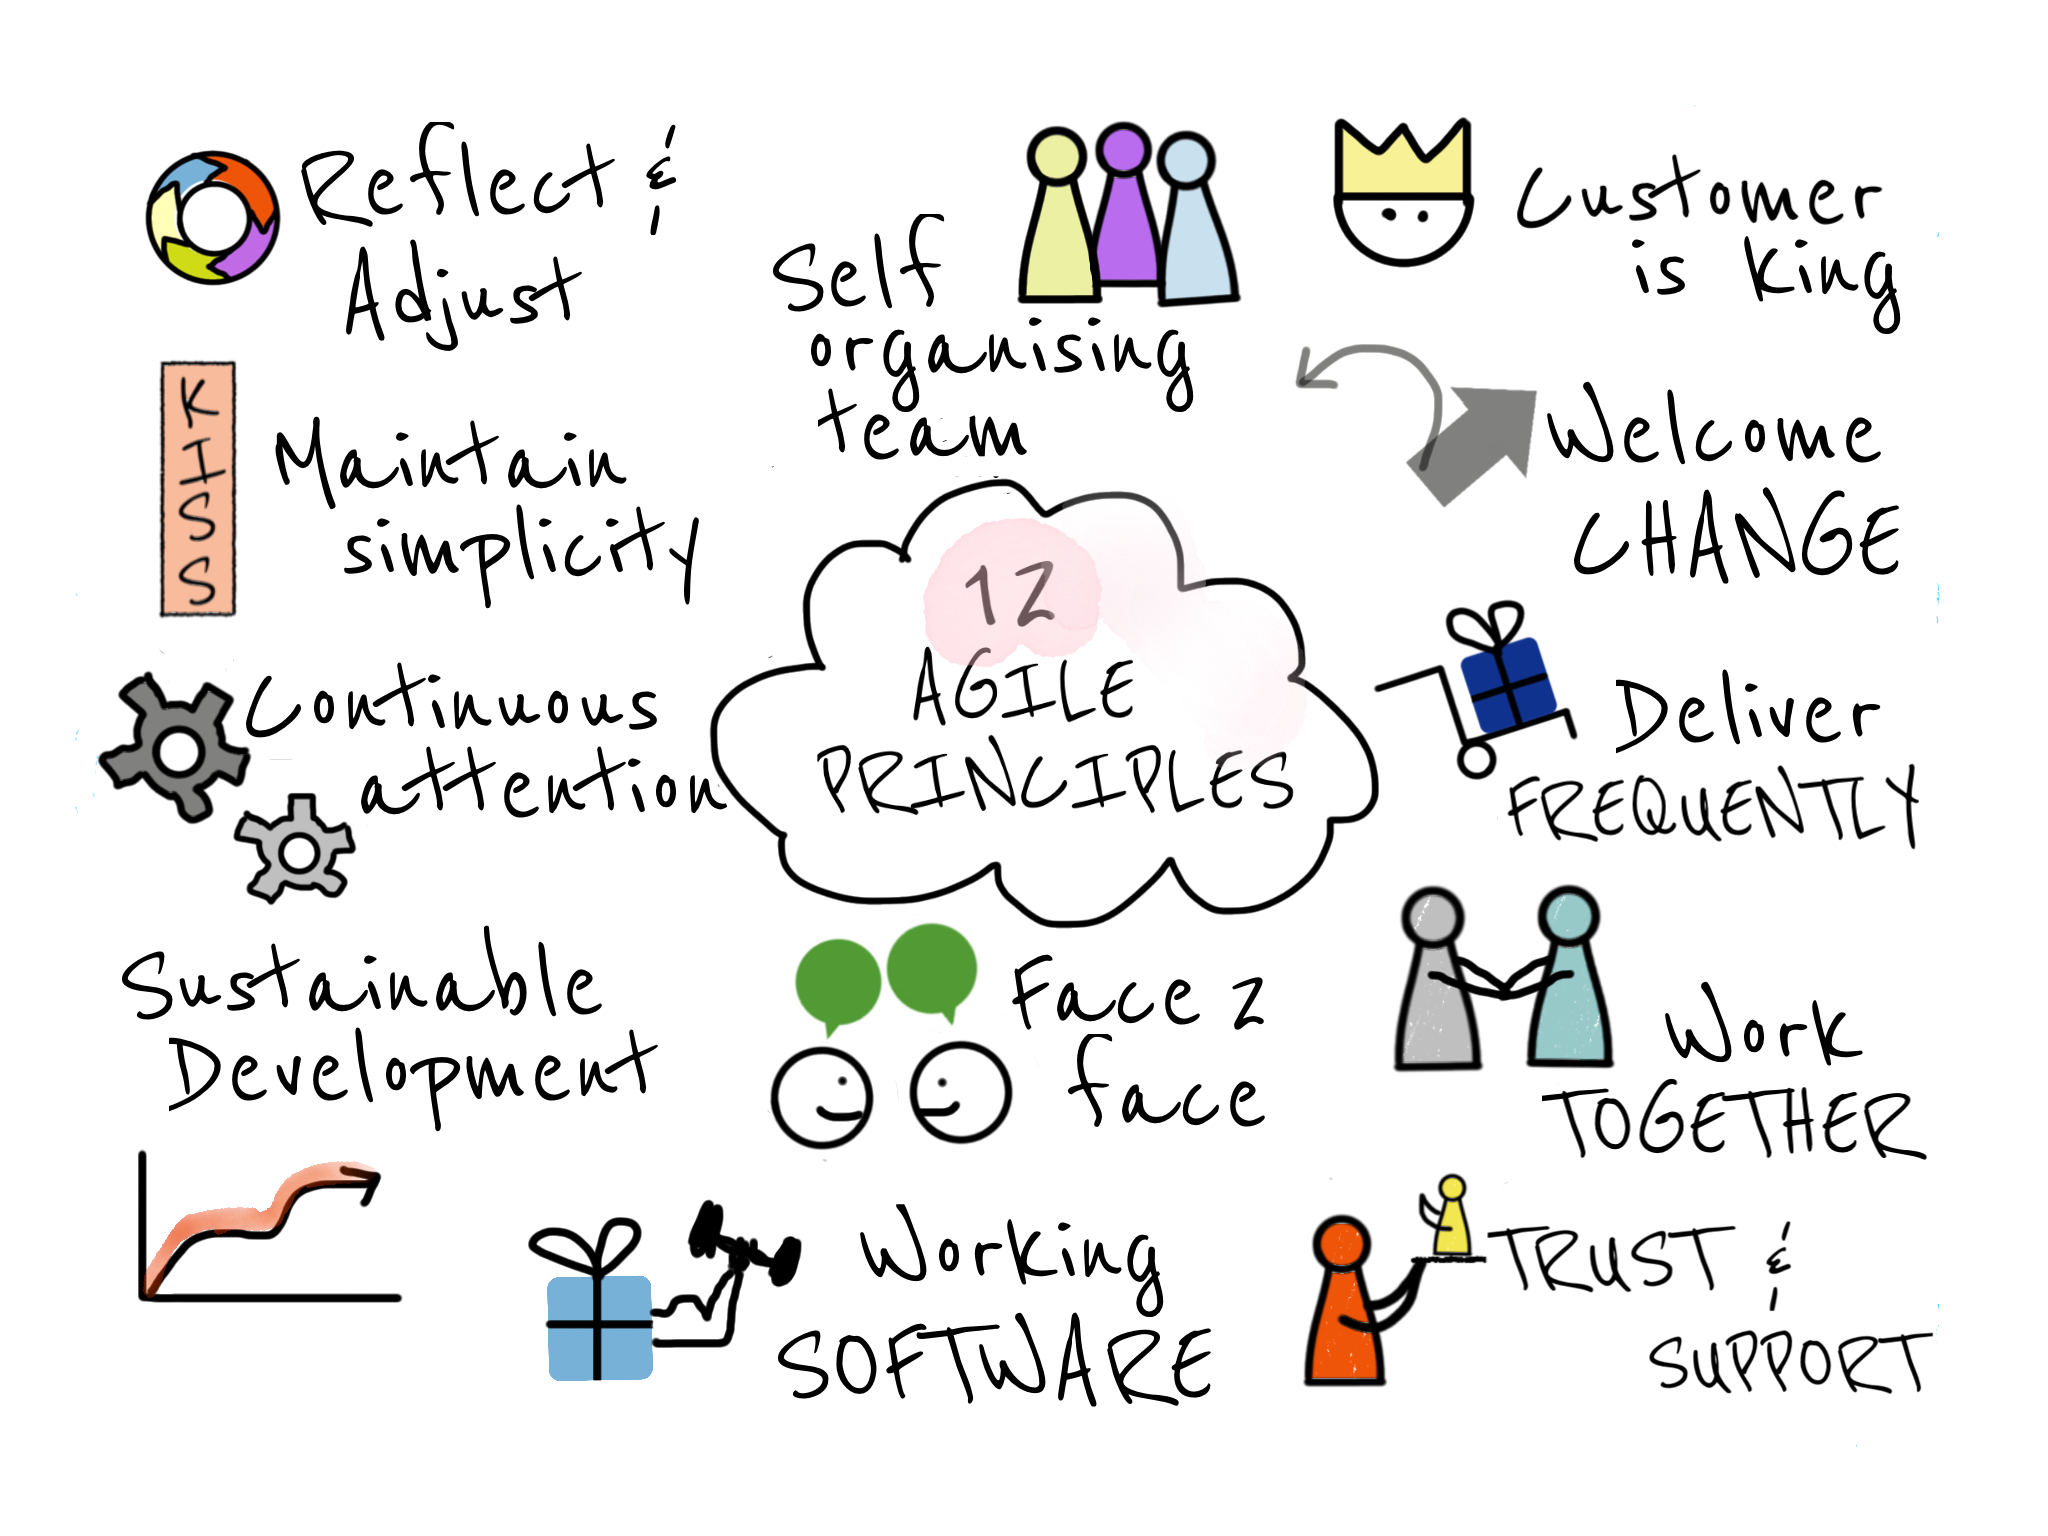
\includegraphics[width=0.3\textwidth]{images/agile-manifesto.png}
        \caption{the 12 Agile Principles}
    \end{figure}
\end{frame}

\begin{frame}{1990s: CVS - Concurrent Versions System}
\begin{columns}
    \begin{column}{0.6\textwidth}
        \begin{itemize}
            \item \textbf{Developed in 1986}, became dominant in 1990s
            \item \textbf{Centralized Architecture}: Single central repository
            \item \textbf{Key Features}:
                \begin{itemize}
                    \item Basic version tracking
                    \item Multiple developer support
                    \item Network-based access
                \end{itemize}
            \item \textbf{Limitations}:
                \begin{itemize}
                    \item No atomic commits
                    \item Poor branching/merging
                    \item Slow network operations
                    \item Single point of failure
                \end{itemize}
        \end{itemize}
    \end{column}
    % \begin{column}{0.4\textwidth}
    %     \includegraphics[width=0.9\textwidth]{images/cvs_architecture.png}
    %     \\\scriptsize{CVS Centralized Architecture}
    % \end{column}
\end{columns}
\begin{block}{}
CVS brought version control to the masses, but collaboration was sequential and cautious.
\end{block}
\end{frame}

\begin{frame}{2000: Subversion - "CVS Done Right"}
\begin{itemize}
    \item \textbf{Created in 2000} by CollabNet to fix CVS limitations
    \item \textbf{Improvements over CVS}:
        \begin{itemize}
            \item \textbf{Atomic commits}: All changes succeed or fail together
            \item \textbf{Better branching/tagging}: Cheap copy operations
            \item \textbf{Versioned directories and renames}
            \item \textbf{Better binary file handling}
        \end{itemize}
    \item \textbf{Still centralized}: Single repository model
    \item \textbf{Adoption}: Quickly became the enterprise standard
    \item \textbf{Limitations}: Central server = single point of failure, offline work difficult
\end{itemize}
% \begin{center}
%     \includegraphics[width=0.5\textwidth]{images/svn_logo.png}
% \end{center}
\end{frame}


\begin{frame}{2002-2005: The BitKeeper Controversy}
\begin{columns}
    \begin{column}{0.6\textwidth}
        \begin{itemize}
            \item \textbf{Linux kernel development} outgrew patch-based workflow
            \item \textbf{BitKeeper}: Proprietary distributed version control system
            \item \textbf{Adopted by Linux in 2002}: Enabled true distributed development
            \item \textbf{Revolutionary features}:
                \begin{itemize}
                    \item Distributed repositories
                    \item Excellent branching/merging
                    \item Fast performance
                \end{itemize}
            \item \textbf{Controversy (2005)}: License disputes led to BitKeeper withdrawal
            \item \textbf{Catalyst}: Forced Linux community to create their own solution
        \end{itemize}
    \end{column}
    \begin{column}{0.4\textwidth}
        % \includegraphics[width=0.9\textwidth]{images/linus_torvalds.jpg}
        % \\\scriptsize{Linus Torvalds, creator of Linux and Git}
    \end{column}
\end{columns}
\end{frame}

\begin{frame}{2005: Git - The Linux Community's Answer}
\begin{itemize}
    \item \textbf{Created by Linus Torvalds in 2005} after BitKeeper controversy
    \item \textbf{Design goals}:
        \begin{itemize}
            \item Distributed and peer-to-peer
            \item Strong cryptographic integrity
            \item Fast branching/merging
            \item Efficient with large projects
            \item Support for non-linear development
        \end{itemize}
    \item \textbf{Key innovations}:
        \begin{itemize}
            \item Content-addressable storage (SHA-1 hashes)
            \item Directed acyclic graph (DAG) for history
            \item Three-stage thinking (working directory, staging area, repository)
        \end{itemize}
\end{itemize}
% \begin{center}
%     \includegraphics[width=0.3\textwidth]{images/git_logo.png}
% \end{center}
\end{frame}

\begin{frame}{Why Git Won: Distributed Workflows}
\begin{columns}
    \begin{column}{0.5\textwidth}
        \textbf{Centralized (CVS/SVN)}
        \begin{itemize}
            \item Single source of truth
            \item Sequential commits
            \item Server required 
            \item Branching is expensive
            \item Linear history
        \end{itemize}
    \end{column}
    \begin{column}{0.5\textwidth}
        \textbf{Distributed (Git)}
        \begin{itemize}
            \item Every clone is a full repository
            \item Parallel development
            \item Work offline, sync later
            \item Cheap branching
            \item Non-linear history
        \end{itemize}
    \end{column}
\end{columns}

\begin{block}{The Game Changer}
Git enabled workflows like \textbf{feature branching} and \textbf{pull requests}, making open-source collaboration scalable.
\end{block}
\end{frame}


\begin{frame}{GitHub and the Social Coding Revolution (2008)}
\begin{itemize}
    \item \textbf{GitHub launched 2008}: Added social layer to Git
    \item \textbf{Key innovations}:
        \begin{itemize}
            \item Pull Requests: Code review as first-class citizen
            \item Fork \& Pull model: Easy contribution to any project
            \item Issues, Projects, Wikis: Integrated project management
        \end{itemize}
    \item \textbf{Network effects}: Made open-source collaboration mainstream
    \item \textbf{Enterprise adoption}: GitHub Enterprise, GitLab, Bitbucket
\end{itemize}
% \begin{center}
%     \includegraphics[width=0.6\textwidth]{images/github_pull_request.png}
%     \\\scriptsize{Pull Request Interface - The Heart of Modern Collaboration}
% \end{center}
\end{frame}

\begin{frame}{Git-Enabled CI/CD: The Automation Revolution}
\begin{itemize}
    \item \textbf{Continuous Integration (CI)}: Automatically build and test every commit
    \item \textbf{Continuous Deployment/Delivery (CD)}: Automatically deploy passing code
    \item \textbf{Git as the trigger}: 
        \begin{itemize}
            \item Push to repository triggers automated pipeline
            \item Branch protection rules enforce quality gates
            \item Pull request status checks prevent bugs
        \end{itemize}
    \item \textbf{Key tools}: Jenkins, GitHub Actions, GitLab CI, CircleCI
\end{itemize}

% \begin{center}
%     \includegraphics[width=0.8\textwidth]{images/git_ci_cd_pipeline.png}
%     \\\scriptsize{Modern Git-triggered CI/CD Pipeline}
% \end{center}
\end{frame}

\begin{frame}{The Evolution Timeline}
\begin{center}
    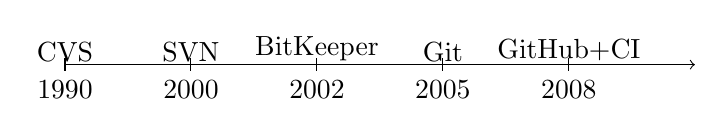
\begin{tikzpicture}[scale=0.8]
        \draw[->] (0,0) -- (10,0);
        \foreach \x/\year/\text in {0/1990/CVS, 2/2000/SVN, 4/2002/BitKeeper, 6/2005/Git, 8/2008/GitHub+CI/CD}
            \draw (\x,0.1) -- (\x,-0.1) node[below] {\year} node[above] {\text};
    \end{tikzpicture}
\end{center}

\begin{itemize}
    \item \textbf{1990s}: Centralized era - sequential collaboration
    \item \textbf{2000s}: Centralized improvement - better but still limited
    \item \textbf{2002-2005}: Distributed awakening - BitKeeper shows the way
    \item \textbf{2005+}: Git revolution - parallel, distributed collaboration
    \item \textbf{2008+}: Social coding + automation - CI/CD ecosystem
\end{itemize}
\end{frame}

\begin{frame}[t]{2010s: AIOps and Cloud Native}
\begin{itemize}
    \item \textbf{AIOps}: Applying AI to operations
    \begin{itemize}
        \item Automated monitoring and incident response
        \item Predictive analytics for system performance
        \item Anomaly detection and root cause analysis
    \end{itemize}
    \item \textbf{Cloud Native Development}
    \begin{itemize}
        \item Microservices architecture
        \item Containerization (Docker, Kubernetes)
        \item Serverless computing
    \end{itemize}
\end{itemize}
\begin{center}
    % Add appropriate image
    % \includegraphics[width=0.6\textwidth]{images/aiops-cloud.png}
\end{center}
\end{frame}

\subsection{LLM Era}

\begin{frame}[t]{2020s: The LLM Revolution}
    \begin{itemize}
        \item \textbf{Large Language Models transform software engineering}
        \item GitHub Copilot (2021) and similar tools
    \end{itemize}
    \begin{figure}
        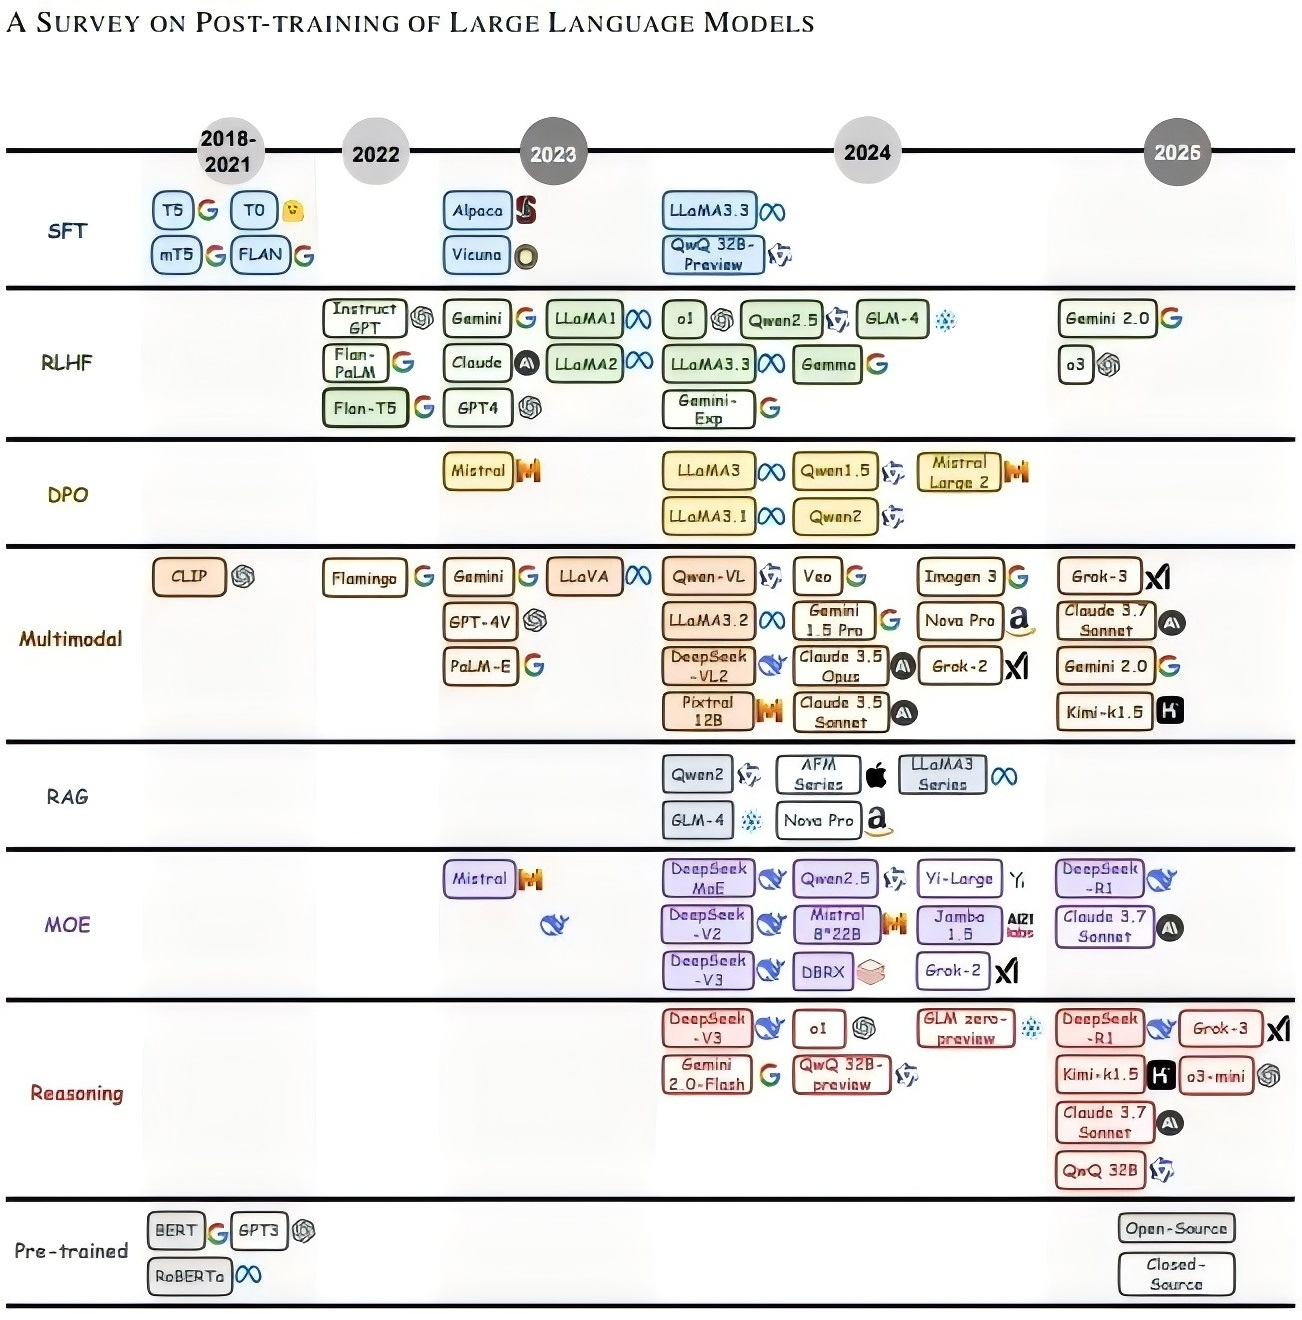
\includegraphics[width=0.5\textwidth]{images/timeline.jpg}
        \caption{Timemline for LLMs}
    \end{figure}
\end{frame}

\begin{frame}[t]{LLM Impact on Software Engineering}
\begin{itemize}
    \item \textbf{Code Generation}: From autocomplete to entire function generation
    \item \textbf{Debugging Assistance}: AI-powered bug detection and fixes
    \item \textbf{Documentation}: Automated documentation generation
    \item \textbf{Code Review}: AI-assisted quality assurance
    \item \textbf{Testing}: Intelligent test case generation
\end{itemize}
\begin{block}{Future Directions}
\begin{itemize}
    \item AI pair programmers becoming standard
    \item New programming paradigms emerging
    \item Focus shifting to prompt engineering and AI supervision
\end{itemize}
\end{block}
\end{frame}

\subsection{Conclusion}


\begin{frame}[t]{Looking Forward}
\begin{itemize}
    \item Continuous evolution from disciplined engineering to AI augmentation
    \item Increasing emphasis on automation and intelligence
    \item The human element remains crucial in system design and oversight
    \item AI is powerful, but it is neither a silver bullet nor an elixir
\end{itemize}
\begin{center}
    \textbf{The journey continues...}
\end{center}
\end{frame}
\section{Brief History of Artificial Intelligence}
\subsection{Pioneering Thoughts}
\begin{frame}[t]{The Seeds of an Idea}
    \begin{itemize}
            % \item \textbf{Ancient Myths}: Stories of artificial beings endowed with intelligence (e.g., Talos, Golems).
            % \item \textbf{Philosophical Foundations}: Descartes' mind-body problem, Hobbes' view of reasoning as calculation.
        \item \textbf{Ada Lovelace (1843)}: Questioned whether machines could originate ideas, or only do what we command.
        \item \textbf{Early 20th Century}: Karel Čapek's play "R.U.R." (1920) coins the term "robot".
    \end{itemize}

    \begin{figure}
        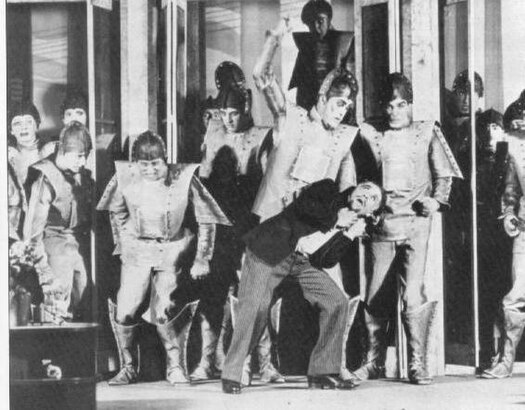
\includegraphics[width=0.3\textwidth]{images/Capek_RUR.jpg}
        \caption{Capek's play R.U.R}
    \end{figure}
\end{frame}
\subsection{1950s: The Birth of a Field}

\begin{frame}[t]{1950s: The Foundational Decade}
    \begin{itemize}
        \item \textbf{Alan Turing (1950)}: Publishes "Computing Machinery and Intelligence", proposing the \textbf{Turing Test}.
    \end{itemize}
    \begin{figure}
        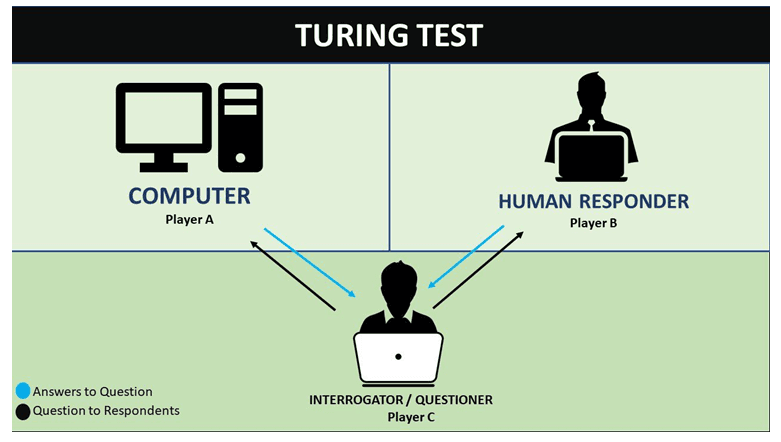
\includegraphics[width=0.7\textwidth]{images/turing-test.png}
        \caption{Diagram of the Turing Test}
    \end{figure}
\end{frame}

\begin{frame}[t]{1950s: The Foundational Decade}
    \begin{itemize}
        \item \textbf{The Name is Coined}: John McCarthy organizes the \textbf{Dartmouth Conference} (1956) and coins the term "Artificial Intelligence".
    \end{itemize}
    \begin{figure}
        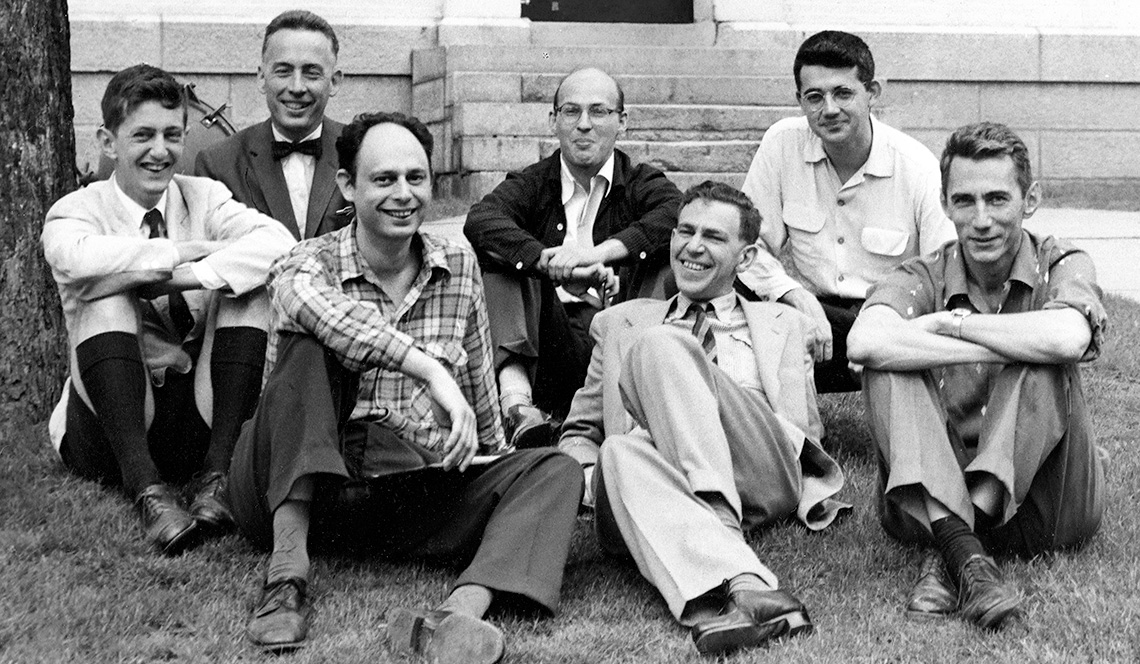
\includegraphics[width=0.7\textwidth]{images/Dartmouth-1956-Conference.jpg}
        \caption{Dartmouth Conference}
    \end{figure}

    \begin{block}{The Goal Was Set}
        "Every aspect of learning or any other feature of intelligence can in principle be so precisely described that a machine can be made to simulate it." - Dartmouth Proposal
    \end{block}
\end{frame}

\subsection{1960s-70s: Symbolic AI and the First AI Winter}

\begin{frame}[t]{1960s-70s: Symbolic AI \& Limits}
\begin{itemize}
    \item \textbf{Symbolic AI (GOFAI)}: Focused on manipulating symbols and logical rules to represent knowledge and solve problems.
    \item \textbf{ELIZA} (1966): An early natural language processing program that simulated a Rogerian psychotherapist.
    % \item \textbf{The Limits}: Symbolic AI struggled with the complexity and ambiguity of the real world. It required massive, hand-coded knowledge bases.
    \item \textbf{The Lighthill Report (1973)}: Criticized AI's failure to meet its grand promises, leading to sharp cut in funding - the \alert{First AI Winter}.
\end{itemize}
\begin{figure}
    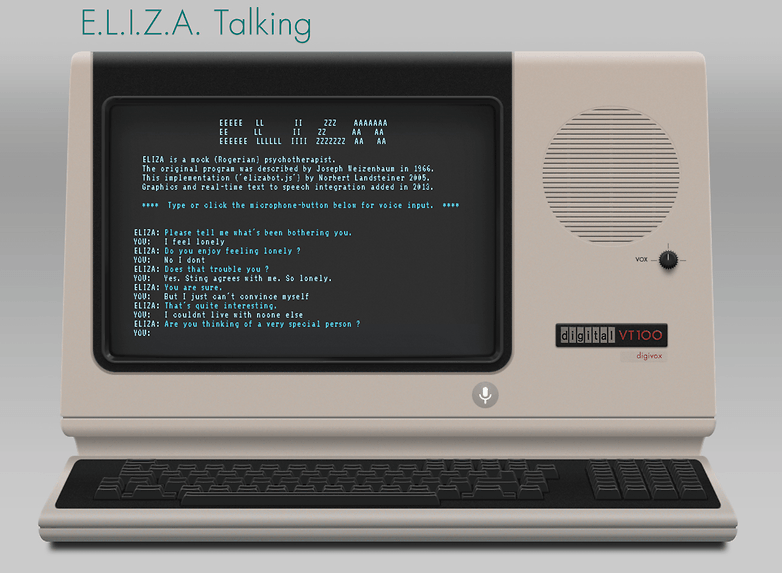
\includegraphics[width=0.4\textwidth]{images/eliza.png}
    \caption{ELIZA}
\end{figure}
\end{frame}

\subsection{1980s: Expert Systems and the Second AI Winter}

\begin{frame}[t]{1980s: The Rise and Fall of Expert Systems}
\begin{columns}
    \begin{column}{0.6\textwidth}
        \textbf{Expert Systems}
        \begin{itemize}
            \item Aimed to capture the knowledge of human experts in rule-based systems.
            \item MYCIN system for diagnosing blood infections performed as well as experts.
        \end{itemize}
        \textbf{The Second AI Winter}
        \begin{itemize}
            \item Expert systems were \alert{brittle}, expensive to maintain, and could not learn.
            \item They failed to scale beyond narrow domains.
            \item By the late 1980s, the hype cycle crashed again, leading to the \textbf{Second AI Winter}.
        \end{itemize}
    \end{column}
    \begin{column}{0.4\textwidth}
        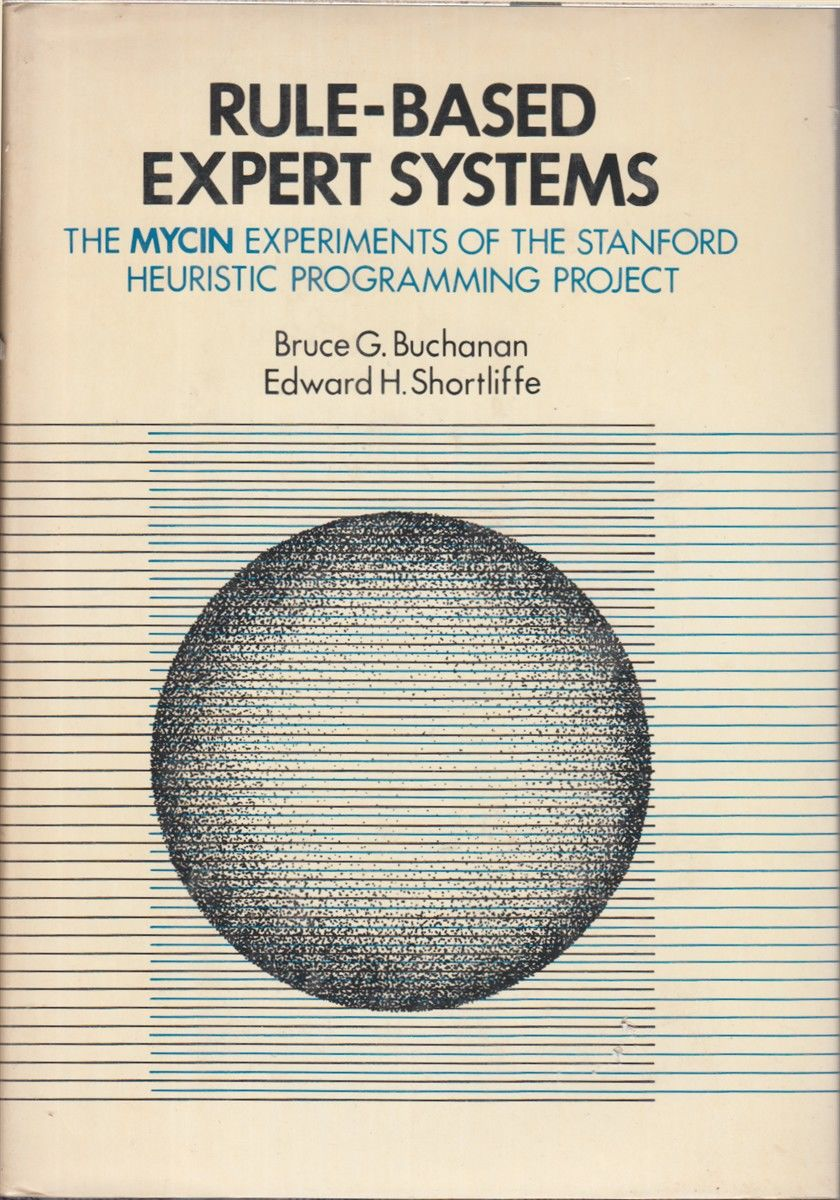
\includegraphics[width=0.9\textwidth]{images/mycin.jpg}
        \\\scriptsize{Rule-Based Expert System}
    \end{column}
\end{columns}
\end{frame}

\subsection{1990s-2000s: The Statistical Turn and Machine Learning}

\begin{frame}[t]{1990s-2000s: A New Paradigm}
\begin{itemize}
    \item \textbf{Shift from Logic to Statistics}: Instead of programming logical rules, researchers focused on creating systems (e.g., SVM, Random Forests) that could \textbf{learn from data}.
    % \item \textbf{The Rise of Machine Learning}:
    %     \begin{itemize}
    %         \item \textbf{Support Vector Machines (SVMs)} and other statistical models became powerful tools.
    %         \item \textbf{The Web} provided vast amounts of data for training.
    %     \end{itemize}
    % \item \textbf{Practical Successes}:
    %     \begin{itemize}
    %         \item \textbf{Spam Filters} using Naive Bayes classifiers.
    %         \item \textbf{Recommendation Systems} (e.g., Amazon, Netflix).
    %         \item \textbf{Search Engines} (e.g., Google's PageRank algorithm).
    %     \end{itemize}
    \item \textbf{IBM Deep Blue (1997)}: Defeated world chess champion Garry Kasparov, a landmark symbolic achievement powered largely by search and evaluation functions.
\end{itemize}
    \begin{figure}
        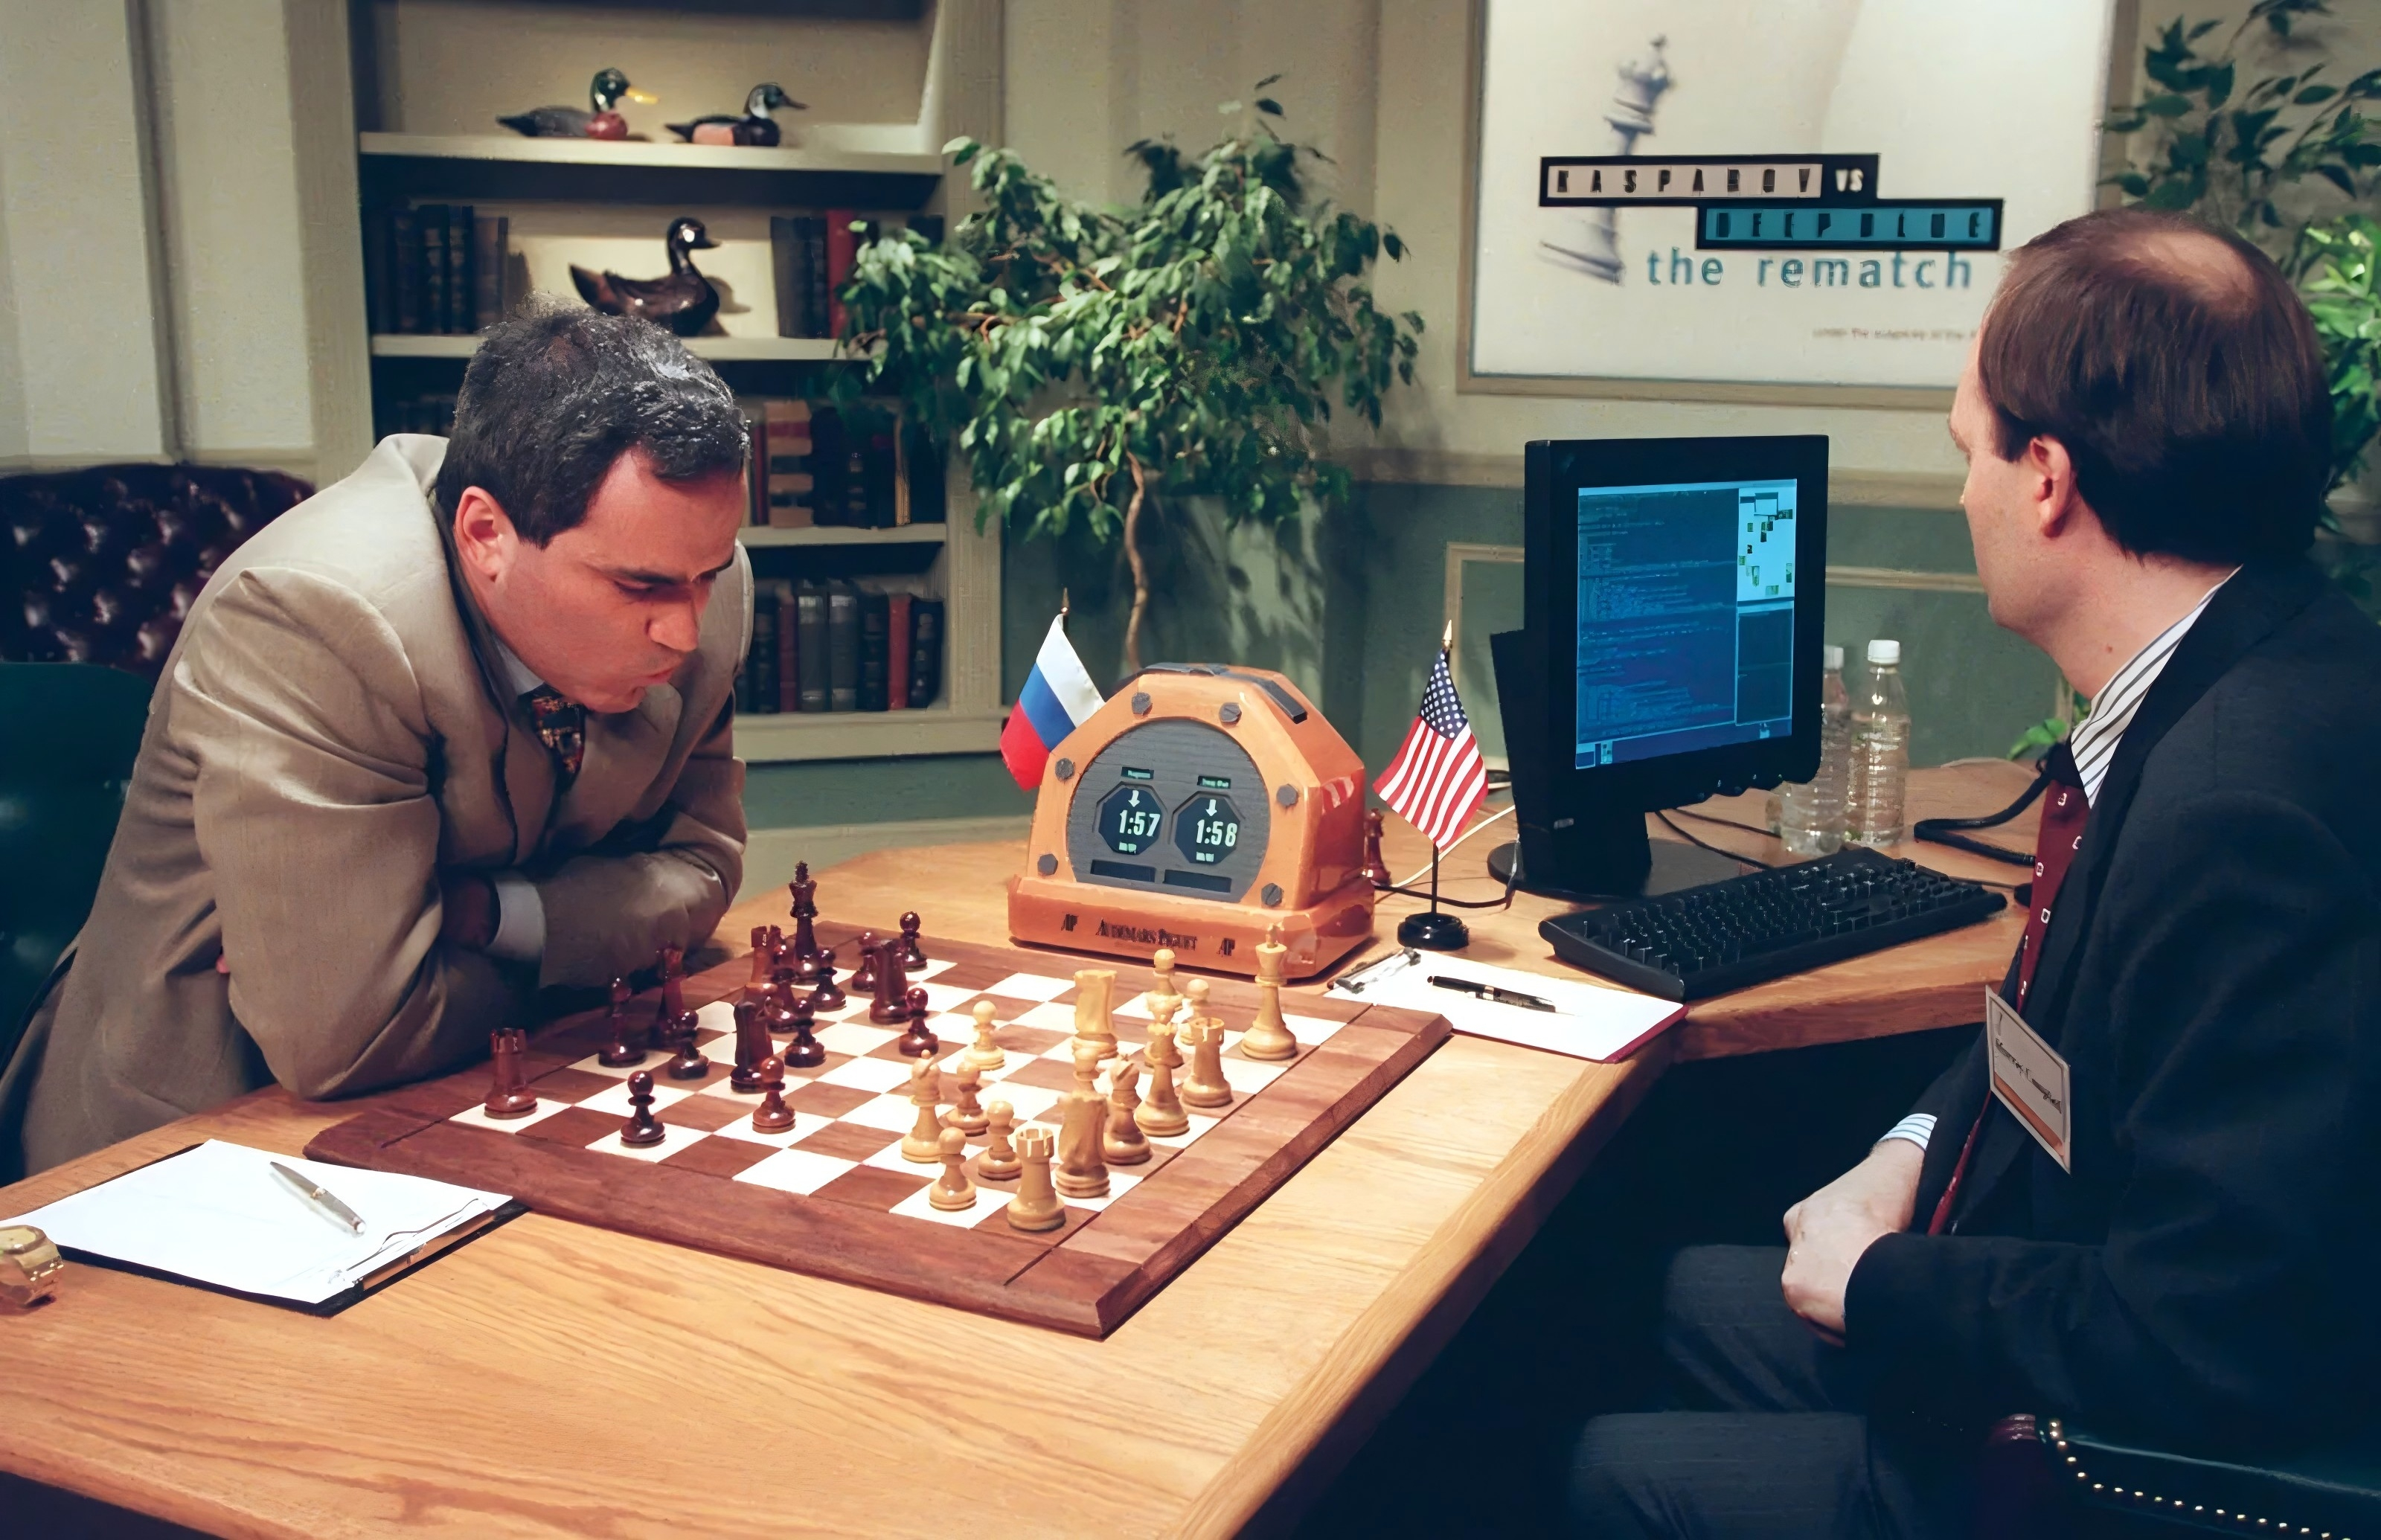
\includegraphics[width=0.5\textwidth]{images/Garry-Kasparov-Deep-Blue-IBM-computer.jpg}
        \caption{Deep Blue vs. Garry Kasparov}
    \end{figure}
\end{frame}

\subsection{2010s: The Deep Learning Revolution}

\begin{frame}[t]{2010s: Deep Learning Unleashed}
        \textbf{The Breakthrough}
        \begin{itemize}
            \item \textbf{Key Enablers}: Massive datasets (Big Data) and powerful parallel processing (GPUs).
            % \item \textbf{ImageNet Competition (2012)}: A deep neural network (AlexNet) drastically reduced error rates, shocking the research community. This was the "big bang" moment for modern AI.
            \item \textbf{The Technique}: \textbf{Deep Learning} uses neural networks with many layers to automatically learn hierarchical features from raw data.
        \end{itemize}
        \textbf{Landmark Achievements}
        \begin{itemize}
            \item \textbf{AlphaGo (2016)}: Defeated the world champion in Go, a game considered far more complex than chess.
        \end{itemize}
        \begin{figure}
            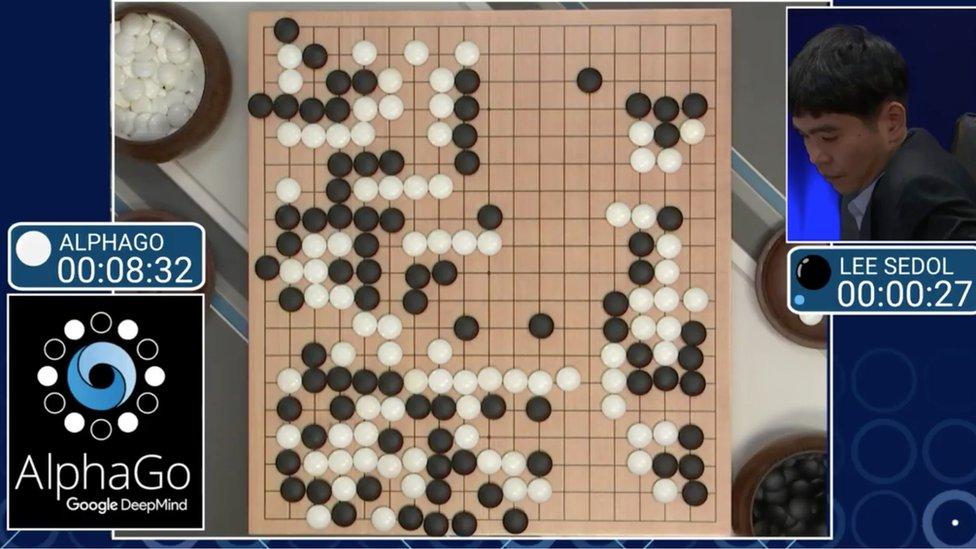
\includegraphics[width=0.5\textwidth]{images/alphago.jpg}
            \caption{AlphaGo vs. Lee Sedol}
        \end{figure}

\end{frame}

\subsection{2020s: The Era of Large Language Models}

\begin{frame}[t]{2020s: The LLM and Generative AI Era}
\begin{itemize}
    \item \textbf{Scale is All You Need}: The discovery that vastly scaling up neural networks (size, data, compute) leads to emergent abilities.
    \item \textbf{The Transformer Architecture (2017)}: Became the foundational model for almost all modern AI, enabling parallel processing of sequences (like text).
    \item \textbf{Large Language Models (LLMs)}:
        \begin{itemize}
            \item Models like GPT-3, GPT-4, Claude, Llama are trained on most of the public internet.
            \item Capable of \textbf{generating human-like text}, translating, summarizing, and coding.
        \end{itemize}
    \item \textbf{Generative AI}: LLMs power tools like ChatGPT, which bring AI capabilities to the general public.
    \item \textbf{Multimodal AI}: Models that can understand and generate across different modalities (text, images, audio).
\end{itemize}
\begin{center}
    % \includegraphics[width=0.7\textwidth]{images/transformer_architecture.png}
\end{center}
\end{frame}

\subsection{Conclusion}

\begin{frame}[t]{AI History: A Journey of Waves}
\begin{center}
    % \includegraphics[width=0.9\textwidth]{images/ai_history_waves.png}
    \scriptsize{The AI field has progressed through waves of optimism followed by "winters" of reduced funding, each wave building on the last.}
\end{center}
\begin{block}{The Pattern}
Symbolic AI (Rules) $\rightarrow$ Statistical ML (Data) $\rightarrow$ Deep Learning (Representations) $\rightarrow$ Generative AI (Creation)
\end{block}
\end{frame}

\begin{frame}[t]{Looking Forward}
\begin{itemize}
    \item \textbf{Artificial General Intelligence (AGI)}: The original, elusive goal of human-level intelligence remains on the horizon.
    \item \textbf{Ethics and Safety}: As AI becomes more powerful, concerns about bias, control, and alignment with human values become paramount.
    \item \textbf{AI as a Commodity}: AI capabilities are being integrated into almost every software product.
    \item \textbf{The Symbiosis}: The future likely involves a close collaboration between human and artificial intelligence, augmenting human capabilities.
\end{itemize}
\begin{center}
    \textbf{The dream of thinking machines is older than computing itself. The journey is far from over.}
\end{center}
\end{frame}

\section{Topics Combining the Two Disciplines}
\begin{frame}[t]{Search-Based Software Engineering}
    % Search-based software engineering (SBSE) applies metaheuristic search techniques such as genetic algorithms, simulated annealing and tabu search to software engineering problems. 
    Many activities in software engineering can be stated as optimization problems. % Optimization techniques of operations research such as linear programming or dynamic programming are often impractical for large scale software engineering problems because of their computational complexity or their assumptions on the problem structure. 
    Researchers and practitioners use metaheuristic search techniques, which impose little assumptions on the problem structure, to find near-optimal or ``good-enough'' solutions\footnote{\url{https://en.wikipedia.org/wiki/Search-based_software_engineering}}.
\end{frame}

\begin{frame}[t]{Mining Software Repositories}
Within software engineering, the mining software repositories (MSR) field analyzes the rich data available in software repositories, such as version control repositories, mailing list archives, bug tracking systems, issue tracking systems, etc. to uncover interesting and actionable information about software systems, projects and software engineering\footnote{\url{https://en.wikipedia.org/wiki/Mining_software_repositories}}.
\end{frame}

\begin{frame}[t]{Empirical Software Engineering}
Empirical software engineering (ESE) is a subfield of software engineering (SE) research that uses empirical research methods to study and evaluate an SE phenomenon of interest. The phenomenon may refer to software development tools/technology, practices, processes, policies, or other human and organizational aspects\footnote{\url{https://en.wikipedia.org/wiki/Empirical_software_engineering}}. % Common research methods used in ESE for primary and secondary research are the following:

\begin{enumerate}
    \item Primary research (experimentation, case study research, survey research, simulations in particular software Process simulation)
    \item Secondary research methods (Systematic reviews, Systematic mapping studies, rapid reviews, tertiary review)
\end{enumerate}
\end{frame}
\begin{frame}[t]{References}
\begin{thebibliography}{10}
\bibitem{nato1968} NATO Software Engineering Conference (1968)
\bibitem{dijkstra1968} Dijkstra, E. W. (1968). "Go To Statement Considered Harmful"
\bibitem{brooks1975} Brooks, F. P. (1975). \textit{The Mythical Man-Month}. Addison-Wesley. % Added reference
\bibitem{thompson1984} Thompson, K. (1984). "Reflections on Trusting Trust"
\bibitem{stallman1983} Stallman, R. (1983). GNU Manifesto
\bibitem{beck2001} Beck, K. (2001). Agile Manifesto
\bibitem{llm2023} Chen, M. et al. (2023). "Evaluating Large Language Models Trained on Code"
\end{thebibliography}
\end{frame}

\end{document}

